\documentclass[a4paper,10pt]{article}


%Using Lines
\usepackage{algorithm}
\usepackage{algorithmic}
\usepackage{amsmath}
\usepackage{relsize}
\usepackage{amsfonts}
\usepackage{amssymb}
\usepackage{mathtools}
\usepackage{graphicx}
\usepackage{epsfig}
\usepackage{color}
\usepackage{mathtools}
\usepackage{tikz}
\usepackage{relsize}
\usepackage{float}
\usepackage{dsfont}
\usepackage{hyperref}
\usepackage[nameinlink]{cleveref}
\newcommand{\bigqm}[1][1]{\text{\larger[#1]{\textbf{?}}}}
\usepackage{tikz,fullpage}
\usetikzlibrary{arrows, petri, topaths}
\usepackage{tkz-berge}
\usepackage[position=top]{subfig}
\usepackage{verbatim}
\usepackage{amsthm}
\usepackage{pgf}
\usepackage{tikz}
\usepackage[utf8]{inputenc}
\usepackage[english]{babel}
\usepackage{breqn}
\usepackage{dsfont}
\usepackage{tabularx}
\usepackage{xcolor}
\usepackage{mdframed}
\usepackage{xspace}


\usetikzlibrary{arrows, automata, backgrounds,snakes}
% End


% define MACROS
\newcommand{\len}{15}
\newcommand{\LPart}{0.4}
\DeclarePairedDelimiter{\ceil}{\lceil}{\rceil}
\DeclarePairedDelimiter{\floor}{\lfloor}{\rfloor}
\newtheorem{theorem}{Theorem}[section]
\newtheorem{corollary}{Corollary}[theorem]
\newtheorem{lemma}[theorem]{Lemma}
\newtheorem*{remark}{Remark}
\newcounter{casenum}
\newenvironment{caseof}{\setcounter{casenum}{1}}{\vskip.5\baselineskip}
\newcommand{\case}[2]{\vskip.5\baselineskip\par\noindent {\bfseries Case \arabic{casenum}:} #1\\#2\addtocounter{casenum}{1}}
\newcommand\rob{\ensuremath{r}\xspace}
\newcommand\opp{\ensuremath{o}\xspace}
\newcommand{\w}{\ensuremath{W}\xspace}
\newcommand{\fcc}{\ensuremath{FCC}\xspace}
\newcommand{\cros}{\ensuremath{CROS}\xspace}
\newcommand{\coos}{\ensuremath{COS}\xspace}
\newcommand{\gn}{\ensuremath{GN}\xspace}
\newcommand{\gf}{\ensuremath{GF}\xspace}
\newcommand{\go}{\ensuremath{GO}\xspace}
\DeclarePairedDelimiter\abs{\lvert}{\rvert}%
\DeclareMathOperator*{\argmax}{arg\,max} % Jan Hlavacek
\allowdisplaybreaks[2]
\newtheorem{definition}{Definition}

\makeatletter
\def\BState{\State\hskip-\ALG@thistlm}
\makeatother
% end


%%%%%% Latex Configuration
\renewcommand{\topfraction}{0.85}
\renewcommand{\textfraction}{0.1}
\renewcommand{\algorithmiccomment}[1]{// #1}
%%%%%
\long\def\symbolfootnote[#1]#2{\begingroup%
\def\thefootnote{\fnsymbol{footnote}}\footnote[#1]{#2}\endgroup}



\begin{document}

\begin{titlepage}
\begin{center}



\includegraphics[width=0.9\textwidth]{Images/logo.jpg}\\[1cm]
\textsc{\LARGE Bar Ilan University}\\[1.5cm]
\textsc{\Large M.Sc Draft}\\[0.5cm]
%\hrule \\[0.4cm]
%{\huge \bfseries Speeding Frontier-Based Exploration by
%Using Semantic Labeling}\\[0.4cm]
%\hrule \\[1.5cm]

\hrule
{ \vspace{2 mm} }
{ \huge \bfseries Competitive Coverage}
{ \vspace{3 mm} }
\hrule
{ \vspace{8 mm} }
% \author{Moshe N. Samson\\
% advised by Noa Agmon\\
% The MAVERICK Group, Computer Science Department\\
% Bar Ilan University\\
% Ramat Gan, Israel 52900\\
% \tt\small samson.moshe@gmail.com

%author and supervisor
\begin{minipage}{0.4\textwidth}
\begin{flushleft} \large
\emph{Author:}\\
Moshe N. Samson 

\end{flushleft}
\end{minipage}
\begin{minipage}{0.4\textwidth}
\begin{flushleft} \large
\emph{Supervisor:} \\
Noa Agmon
\end{flushleft}
\end{minipage}


\vfill


\large{The SMART Group, Computer Science Department\\
Bar Ilan University\\
Ramat Gan, Israel 52900\\
\tt\small samson.moshe@gmail.com}

\vfill

\today

\end{center}
\end{titlepage}

%opening
\title{Competitive Coverage}
\author{Moshe N. Samson\\
advised by Noa Agmon\\
The SMART Group, Computer Science Department\\
Bar Ilan University\\
Ramat Gan, Israel 52900\\
\tt\small samson.moshe@gmail.com
}



\tableofcontents
\maketitle

\section{Introduction}
The robotic coverage problem is one of the fundamental problems in robotic research, and as such has received considerable attention in the past two decades \cite{galceran2013survey}. The problem has its theoretical interest, but is of special interest due to its immediate applicability in real world settings, such as cleaning, coating, demining and search and rescue. 

In the original problem of robotic coverage, a robot's goal is to determine a path that will visit each point in a given area at least once, usually while minimizing the time for completion \cite{galceran2013survey}. The problem has been examined in different settings, for example offline vs. online coverage \cite{gabriely2001spanning,agmon2008giving}, where the environment map is given in advance or discovered during the execution (respectively), coverage with the presence of threats that might stop the robot \cite{yehoshua2014safest}, and continuous vs. discrete domains \cite{gabriely2001spanning,yang2004neural}. In the multi-robot coverage problem, the coverage is a collaborative effort: each point in the area should be visited at least once by some robot from the team, and the common goal is to minimize the maximal working time of some robot from the team. 

In this work we formally define a new variant of the coverage problem, {\em competitive coverage}, in which robots do not work collaboratively, but competitively. More formally, two robots, \rob and \opp, are to cover a given area represented as a grid, and our goal is to maximize the number of cells \rob covers first, before they are covered by \opp.

The problem can be classified as {\em symmetric} or {\em asymmetric}, which refers to wither \opp even knows about \rob's existence or not, regardless to what is the extent of such information. In this work we examine in depth the {\em asymmetric} variant of the problem, in which \opp operates without the knowledge of \rob's existence, and \rob knows it should compete with \opp. The problem is also modeled by the level of information one robot has on the other (beside its existence): initial location and strategy/coverage-path. We consider four different models: (i) \rob knows the initial location of \opp and its planned coverage path ; (ii) \rob knows only the path, but does not know \opp's initial location ; (iii) \rob knows \opp's initial location, but not its coverage path ; (iv) \rob does not know both \opp's path and its location.

Solving the competitive coverage problem, in some cases, is as computationally hard as solving the original coverage problem \cite{arkin2000approximation}. For the sake of the analysis, we consider environments in which an optimal coverage path can be computed in polynomial time, for example by using the Spanning-Tree Coverage Algorithm \cite{gabriely2001spanning}, which generates, cyclic coverage paths under some assumptions on the environment. 

We therefore present an optimal algorithm for \opp in the full-information case, and show that, surprisingly, having some information is equivalent (in the average case) to having no information at all. That is, if \rob has information only on \opp's location {\em or} on its path, its optimal behavior is exactly as if it does not know any of those. We support our theoretical analysis with ROS/Gazebo simulation, demonstrating our findings. 

\section{Related Work}
The problem of single-robot coverage has been extensively discussed in the literature, and many approaches to coverage path planning have been developed though the years. In \cite{galceran2013survey} Galceran and Carreras offer a recent survey of coverage path planning methods.

The coverage problem can be classified as either offline or online. 
Online algorithms assumes zero or partial knowledge regarding the world to be covered, and the coverage-path is generated while advancing in that world. Conversely, Offline algorithms rely on stationary, known beforehand map of the world, and thus create the full coverage-path before even starting to move through it. In this work, we focus on offline coverage.

The coverage problem has been reduced to the traveling salesman problem \cite{arkin2000approximation}, and thus known to be $\mathcal{NP}$-complete even on simple graphs such as grid graphs \cite{papadimitriou1977euclidean}. However, there are known solutions to the coverage problem, that work even in linear time. For example, the offline algorithm STC, presented in \cite{gabriely2001spanning} has been proven to be optimal on discrete world, computes an optimal covering path in linear time $O(N)$, where $N$ is the number of cells comprising the approximate area. In our work we considered an approximate cellular decomposition (as explained in \cite{galceran2013survey}) into finite grid, and thus we know there exists an optimal coverage path which can be found in a linear time.

A considerable attention has been given in the literature also to the multi-robot variant of the coverage problem. In multi-robot coverage, multiple robots work in coordination in order to jointly cover an area. The robots can be with or without leader(s), relying on full or limited communication (e.g., \cite{agmon2008giving}), in online or offline manner \cite{agmon2008giving, de2005blind}.
In this work we do consider multiple (exactly 2) robots, but working noncooperately, one on each side.

Yehoshua et al. \cite{yehoshua2013robotic} recently introduced a new variant of the coverage problem, in which the covering robots operate in an adversarial environment, where threats exist and might stop the robot. Online algorithms for adversarial coverage were discussed in  \cite{yehoshua2015online}, and multi-robot algorithms for adversarial coverage were discussed in \cite{yehoshua2016multi}.
In this work other robots considered as competitors, and are not being a threat to our robot. %The robot does/doesn not have a behavior to meeting with its opponent, but in any case, it does not make it stop.

Another worth-mentioning niche relating to coverage is the patrolling task, in which the robot(s) are to repeatedly visit the area in order to monitor change in state. Most Patrol algorithms are either partition-based, where the area is divided into sub-areas, and each one is assigned to a robot (e.g., \cite{guo2004towards}, \cite{guo2004coverage}, \cite{jung2002tracking}), or are cyclic-based, where all robots travel through one cyclic path, coordinately \cite{chevaleyre2004theoretical}. 
In adversarial patrolling (\cite{agmon2011multi}, \cite{sless2014multi}, \cite{agmon2008multi}), there is an adversary trying to penetrate through the patrol path, undetected. In this work we consider competitors, where both are already in the area, and are trying to visit it as fast as possible. %Also, in patrolling, the enemy is trying (most of the time) to avoid from being detected, while in this work, the other opponent does not necessarily is trying to hide: its concern is different from the one in the Patrol problem.

Finally, the competitive problem is related to the foraging problem, which is searching, and when found, transporting objects to one or more collection points. In \cite{winfield2009foraging} we find a fairly extensive survey of the subject, including defining and describing the principles of foraging, presents the essentials design features that are a requirement for any foraging robot, and presents strategies for multi-robot foraging. \cite{winfield2009foraging} uses Finite-State-Machine to describe the states that constitute foraging. In our work, the robot does not need find anything, therefore there is not the notion of 'capacity' (that exists in foraging), and the choice to go back to certain points depends on the covering strategy assumptions (which, in our case, says that only position visited more than once is the initial position).
%2-3 pages

\section{Competitive Coverage: Definition}
Let \rob and \opp be two robots operating in an obstacle-free grid \w of size $N=m \times n$. Both robots move in the four basic directions (North, South, East, West). Consider \rob to be our robot-of-interest, and \opp to be the opponent. 
The goal of each robot is to cover the area, that is, find a path (denoted as the coverage path) that visits  each point in the area at least once. We define a coverage strategy of a robot as the coverage path, including the order of cells visited (specifically in a cyclic coverage path, the strategy indicates both the cells' ordering, and the direction of movement---clockwise or counterclockwise), or a behavior (for example: opponent chooses randomly, at each step, one of its four neighbors, and go there). We denote \rob's and \opp's strategies by $S_\rob,S_\opp\in \mathcal{S}$, respectively, where $\cal{S}$ stands for the possible strategies space. In the offline version of the competitive coverage problem, $S_\rob$ and $S_\opp$ are computed in advance (before the execution), and mostly consist of cells permutation, where in the online problem, the strategies are behaviors, able to adjust online to the environment.

\opp is covering \w using an optimal coverage strategy, that is, it follows a path guaranteeing coverage in minimal time (we based our experiments on the Spanning-Tree Coverage algorithm \cite{gabriely2001spanning}). \rob's goal is to cover as many cells as possible from \w {\em before they are visited by \rob}. The calculation of the covering strategy of \rob, $S_\rob$, is based on its initial location, $i_r$. The initial position of \opp, $i_\opp$, is not necessarily known to \rob.

The way we define the problem, \rob can be given $i_\opp$, $S_\opp$, both or neither. These types of information are called {\em Information Models}, and defined as follows:
\begin{definition}[\textbf{Information Model}]
Information Model $IM \in \lbrace \varnothing, \lbrace S,I\rbrace \rbrace$, represents the knowledge a robot has on its opponent, where $S\in \mathcal{S} \cup \lbrace S_\emptyset \rbrace$, where $S_\emptyset$ stands for an unknown strategy, and $I \in W \cup \lbrace \w_\emptyset \rbrace$, where $\w_{\emptyset}$ refers to an unknown initial point.
If $IM=\varnothing$ then the player of interest does not know its opponent exists.
Let $IM_\rob$ be the information model \rob is given about \opp, and let $IM_\opp$ be the information model \opp is given about \rob.
\end{definition}
\rob thrives first to maximize the number of cells it covers before \opp. Denote this value by 
\begin{dmath*}[compact]
\fcc_{x}= 
\# \lbrace \textnormal{ Cells First Covered by } x \in \lbrace\rob,\opp\rbrace \rbrace 
\end{dmath*}
When deciding between options with the same \fcc value, \rob will choose the one that yields the fastest world's coverage time - the time it takes \rob to covers all of \w.

\opp can operate with or without the knowledge of \rob's existence. We refer to these cases as the {\em symmetric and asymmetric competitive coverage}, respectively.
In the {\em asymmetric} case, $IM_\opp=\varnothing$, and in the {\em symmetric} case, $IM_\opp \neq \varnothing$. In both, $IM_\rob \neq \varnothing $.

Considering all we said above, we define the competitive coverage problem:
\begin{mdframed}[backgroundcolor=gray!20] 
\begin{definition}[\textbf{Competitive Coverage Problem}]
Let \w be a finite, obstacles-free grid of size $N$. Given $IM_\opp=\lbrace S_\opp ,i_\opp \rbrace$ to \rob and $IM_\rob \in \lbrace \varnothing, \lbrace S_\rob, i_\rob \rbrace \rbrace$ to \opp, find $S_\rob^\star \in \mathcal{S}$ s.t.
\begin{dmath*}[compact]
S_\rob^\star =\argmax_{S_\rob\in\mathcal{S}} \lbrace \fcc_{r}(S_\rob, S_\opp, i_\rob, i_\opp ) \rbrace
\end{dmath*}
\end{definition}
\end{mdframed}

\section{1D World}

There are 4 base problems to answer to when considering the 1D problem, regarding our initial knowledge over the problem:

\begin{enumerate}
\item $i_{\opp}$ is known, $S_{\opp}$ is known
\item $i_{\opp}$ is known, $S_{\opp}$ is not known
\item $i_{\opp}$ is not known, $S_{\opp}$ is known
\item $i_{\opp}$ is not known, $S_{\opp}$ is not known
\end{enumerate}

For each of these problems, we would like to know what is the best strategy for \rob to play.

Let us assume we have 2 major strategies:

$GoNear(\gn)$ - go toward the nearer edge first, until reaching it or meeting the opponent, then turn around and go all the way toward the far edge.

$GoFar(\gf)$ - go toward the far edge first, until reaching it or meeting the opponent, then turn around and go all the way toward the far edge.

And, for cases where its available and relevant, let us define:

$Go(to)Oppenet(\go)$ - go toward the opponent's initial position first, and when meeting, turn around and cover toward the edge until reaching it.

\subsection{Problems 1 and 2} \label{subsections: full and partial information, 1D world}
\begin{lemma}
Assume that $ S_\opp=\gf$ and $i_\opp \in (0,i_\rob)$, then {\rob}s best response is $S_\rob=\gn$.
\end{lemma}
\begin{proof}
Let us compute the expected profits for either strategy for \rob.
If $S_{\rob}=\gf$ then $E=d-r$, and if $S_{\rob}=\gn$ then $E=\frac{(r-o)}{2} + (d-r)$. Since $r > o$ then the expected profits for strategy $S_{\rob}=\gn$ is greater. Illustrations follows:
\end{proof}

\begin{lemma}
Assume that $ S_\opp=\gn$ and $i_\opp \in (i_\rob, N/2)$, then {\rob}s best response is $S_\rob=\gf$.
\end{lemma}
\begin{proof}
Let us compute the expected profit for either strategy for \rob. If $S_{\rob}=\gn$, then both players are moving right. Since \rob will cover all the distance between the players initial positions before meeting \opp, then its expected profit is: $E=o-r+r=o$. On the other hand, if $S_{\rob}=\gn$, then \rob is reaching to the near edge first, turning around, going until meeting \opp. Notice that the distance \rob covers until reaching \opp initial position is $r+o$, which is clearly smaller than what \opp need to cover to reach its initial position again (recall \opp range that we are talking about..). Therefore, the expected profit is; $E=r+o-r=o$.

So, we can say that it is best to $\gf$, in an empty way, and it is true since both options are the same in the manner of the expected profit.
\end{proof}

\begin{lemma}
Let us assume that $S_{\opp}=\gn$ and $o\in\left(\frac{d}{2},d\right)$. Then, \rob best strategy is playing $\gf$.
\end{lemma}
\begin{proof}
Let us compute the expected profits for either strategy for \rob.
If $S_{\rob}=\gn$ then $E=r+\frac{o-r}{2}$. If $S_{\rob}=\gn$, then $E=r+\max\left(0,\frac{o-3r}{2}\right)$. Since $\frac{o-r}{2} > \max\left(0,\frac{o-3r}{2}\right)$ then the expected profits for strategy $S_{\rob}=\gn$ is greater. Illustrations follows:
\end{proof}

\begin{theorem}
If \opp is going toward \rob, the best thing \rob can do is to go toward \opp until meeting, then turn around and go all the way to the edge. In terms of strategy: if $0<o<r$ then $S_{\rob}=\gn$ and if $r<o<d$ then $S_{\rob}=\gn$.
\end{theorem}
\begin{proof}
Follows directly from lemmas 4.1 to 4.3.
\end{proof}

\begin{lemma}
Let us assume that $S_{\opp}=\gn$ and $o\in\left(0,r\right)$ . Then, \rob best strategy is playing \gn.
\end{lemma}
\begin{proof}
Let us compute the expected profits and decide:
if \rob is playing \gn, then the expected profit is: $E=\frac{2}{3}(r-o) +\frac{1}{3}(2o+\frac{r-3o}{2}) + (d-r)$, while if $S_{\rob}=\gn$, then the expected profit is just $(d-r)$. Therefore, it is more profitable for \rob to play \gn than $\gf$.
\end{proof}

\begin{lemma}
Assume that $ S_\opp=\gf$ and $i_\opp \in (N/2,N)$, then {\rob}s best response is $S_\rob=\gf$.
\end{lemma}
\begin{proof}
If $S_{\rob}=\gn$, then both players are moving left at first, and the expected profit is: $E=r+\max\left(\frac{o-3r}{2},0\right)$, and if $S_{\opp}=\gn$, then both players are going toward each other, and then turn around and go toward the far edge, and in this case the expected profit is: $E=\frac{o-r}{2}+r$. Since always $\frac{o-r}{2}>\max\left(\frac{o-3r}{2},0\right)$, then it is always better for \rob to play $\gf$ instead of \gn.
\end{proof}

\begin{lemma}
Let us assume that $S_{\opp}=\gn$ and $o \in \left(\frac{d}{2},d\right)$ . Then, \rob best strategy is playing $\gf$.
\end{lemma}
\begin{proof}
First, consider the case on which $S_{\rob}=\gn$. In this case, both the players start by going right, until \opp turns around. Then the players go toward each other, until they meet.
Notice that after \opp moved from its position to the right edge and it is going back, we have two options: either \opp is reaching its initial position before meeting \rob, and when it hasn't, which means that \rob reached \opp's initial position before \opp (See Figure X).

We can write \rob's profit by:\[E=\begin{cases}
r+\frac{2d-r-o}{2},&2d+r-3o<0\\
p2,&2d+r-3o>0\\
\end{cases}\]

Where the probabilities came from the fact that the first case happen when there is a space from when \opp reached its initial position, until meeting with \rob, happens only when $r+2(d-o) < o$. From this, we extract the probabilities as denoted above.

On the other hand, assume that $S_{\rob}=\gn$. We divide the expected profit into 4 different cases, with probabilities and profits.

\begin{caseof}
  \case{\textsc{Meeting position} $ < r$}{
  \begin{figure}
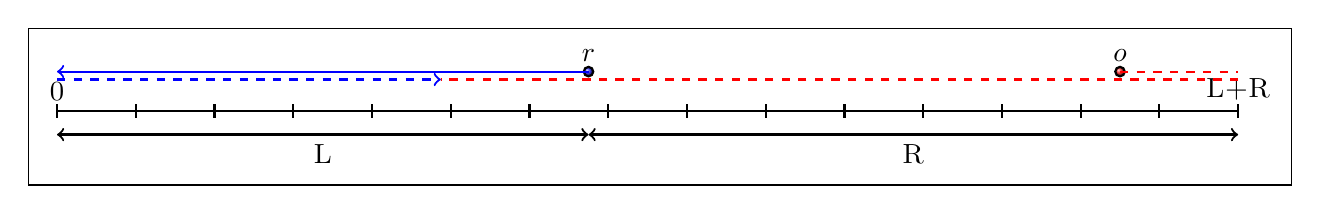
\begin{tikzpicture}[thick,framed]
%draw players
  \draw (0,0) -- (\len,0);
  \draw[snake=ticks,segment length=1cm] (0,0) -- (\len,0);
  \node[above] at (0,0) {$\textsc{0}$};% label the hinge
  \node[above] at (\len,0) {$\textsc{L+R}$};% label the hinge
  
  \filldraw[ball color=blue!80,shading=ball] (0.45*\len,0.5) circle
        (0.06cm) node[above]{\rob};% p1
  
  \filldraw[ball color=red!80,shading=ball] (0.9*\len,0.5) circle
        (0.06cm) node[above]{\opp};% p2
     
   % draw path
   \draw[->, blue] (0.45*\len,0.5) -- (0.0*\len,0.5)
	  	node[pos=0.7,above]{}; % path1 p2
    \draw[->, blue, dashed] (0.0*\len,0.4) -- (0.325*\len,0.4)
	  	node[pos=0.7,above]{}; % path1 p2
   
   \draw[-, red, dashed] (0.9*\len,0.5) -- (\len,0.5)
	  	node[pos=0.5,above]{}; % path1 p1
   \draw[-, red, dashed] (\len,0.4) -- (0.325*\len,0.4)
	  	node[pos=0.5,above]{}; % path1 p1
   
   % draw axis
   \draw[<->] (0, -0.3) -- (0.45*\len, -0.3)
        node[pos=0.5,below]{$\textsc{L}$}; % Left hand
   \draw[<->] (0.45*\len, -0.3) -- (\len, -0.3)
        node[pos=0.5,below]{$\textsc{R}$}; % Right Hand
\end{tikzpicture}
\caption{Case 1}
\end{figure}
\underline{Happen When:} Since the path \rob is doing should be greater than \opp's, it needs to holds that: $2p1>(d-o)+(d-p1)\rightarrow 2d-3r-o<0$.

\underline{Profit:}
The gain here is very simple to deduct from the illustrations: $\abs*{r}$.
}
  \case{$r < \textsc{Meeting position} < o$, \rob turns first}{
  \begin{figure}
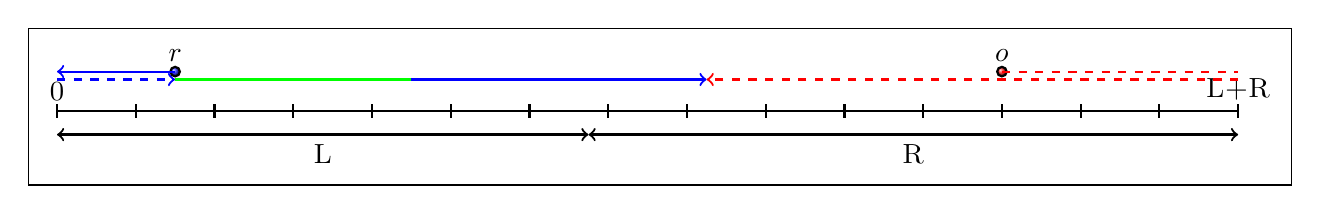
\begin{tikzpicture}[thick,framed]
%draw players
  \draw (0,0) -- (\len,0);
  \draw[snake=ticks,segment length=1cm] (0,0) -- (\len,0);
  \node[above] at (0,0) {$\textsc{0}$};% label the hinge
  \node[above] at (\len,0) {$\textsc{L+R}$};% label the hinge
  
  \filldraw[ball color=blue!80,shading=ball] (0.1*\len,0.5) circle
        (0.06cm) node[above]{\rob};% p1
  
  \filldraw[ball color=red!80,shading=ball] (0.8*\len,0.5) circle
        (0.06cm) node[above]{\opp};% p2
     
   % draw path
   \draw[->, blue] (0.1*\len,0.5) -- (0.0*\len,0.5)
	  	node[pos=0.7,above]{}; % path1 p2
   \draw[->, blue, dashed] (0.0*\len,0.4) -- (0.1*\len,0.4)
	  	node[pos=0.7,above]{}; % path1 p2
   \draw[-, green] (0.1*\len,0.4) -- (0.3*\len,0.4)
	  	node[pos=0.7,above]{}; % path1 p2
   \draw[->, blue] (0.3*\len,0.4) -- (0.55*\len,0.4)
	  	node[pos=0.7,above]{}; % path1 p2
   
   \draw[-, red, dashed] (0.8*\len,0.5) -- (\len,0.5)
	  	node[pos=0.5,above]{}; % path1 p1
   \draw[->, red, dashed] (\len,0.4) -- (0.55*\len,0.4)
	  	node[pos=0.5,above]{}; % path1 p1
   
   % draw axis
   \draw[<->] (0, -0.3) -- (0.45*\len, -0.3)
        node[pos=0.5,below]{$\textsc{L}$}; % Left hand
   \draw[<->] (0.45*\len, -0.3) -- (\len, -0.3)
        node[pos=0.5,below]{$\textsc{R}$}; % Right Hand
\end{tikzpicture}
\caption{green is the extra part \rob is doing before \opp is reaching its initial position}
\end{figure}
  \underline{Happen When:} Since \rob turns before \opp, it holds that $r<d-o$. Also, if they meet between the two players, the case should hold: $r+(2(d-o)-2r)<o\rightarrow 2d-3o-r<0$.

\underline{Profit:} The gain in this case is consists of the $\abs*{r}$ to the left, then going the distance from \rob initial position until \opp is reaching its initial position. Then, its half the left distance. That is: $r+(2d-2o-2r)+\frac{o-(2d-2o-2r)}{2}=\abs*{\frac{2d-r-o}{2}}$
}
  \case{$r < \textsc{Meeting position} < o$, \opp turns first}{
  
  \begin{figure}[H]
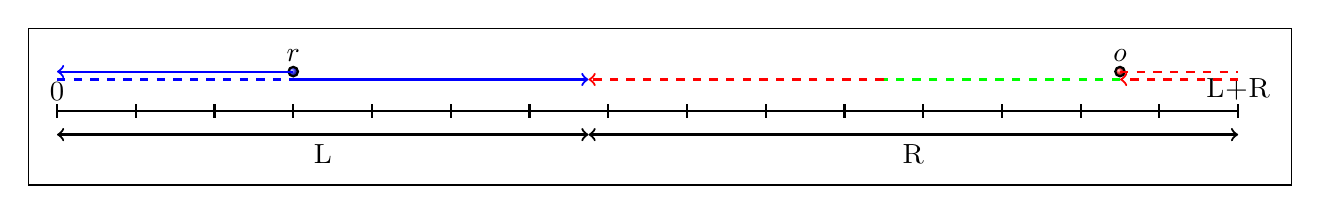
\begin{tikzpicture}[thick,framed]
%draw players
  \draw (0,0) -- (\len,0);
  \draw[snake=ticks,segment length=1cm] (0,0) -- (\len,0);
  \node[above] at (0,0) {$\textsc{0}$};% label the hinge
  \node[above] at (\len,0) {$\textsc{L+R}$};% label the hinge
  
  \filldraw[ball color=blue!80,shading=ball] (0.2*\len,0.5) circle
        (0.06cm) node[above]{\rob};% p1
  
  \filldraw[ball color=red!80,shading=ball] (0.9*\len,0.5) circle
        (0.06cm) node[above]{\opp};% p2
     
   % draw path
   \draw[->, blue] (0.2*\len,0.5) -- (0.0*\len,0.5)
	  	node[pos=0.7,above]{}; % path1 p2
   \draw[-, blue, dashed] (0.0*\len,0.4) -- (0.2*\len,0.4)
	  	node[pos=0.7,above]{}; % path1 p2
   \draw[->, blue] (0.2*\len,0.4) -- (0.45*\len,0.4)
	  	node[pos=0.7,above]{}; % path1 p2
   
   \draw[-, red, dashed] (0.9*\len,0.5) -- (\len,0.5)
	  	node[pos=0.5,above]{}; % path1 p1
   \draw[->, red, dashed] (\len,0.4) -- (0.9*\len,0.4)
	  	node[pos=0.5,above]{}; % path1 p1
   \draw[-, green, dashed] (0.9*\len,0.4) -- (0.7*\len,0.4)
	  	node[pos=0.5,above]{}; % path1 p1
   \draw[->, red, dashed] (0.7*\len,0.4) -- (0.45*\len,0.4)
	  	node[pos=0.5,above]{}; % path1 p1
   
   % draw axis
   \draw[<->] (0, -0.3) -- (0.45*\len, -0.3)
        node[pos=0.5,below]{$\textsc{L}$}; % Left hand
   \draw[<->] (0.45*\len, -0.3) -- (\len, -0.3)
        node[pos=0.5,below]{$\textsc{R}$}; % Right Hand
\end{tikzpicture}
\caption{green is the extra part \opp is doing before \rob is reaching its initial position}
\end{figure}
\underline{Happen When:} This is similar to the second case; Since \opp turns before \rob, then the case should that $d-o<r$. Also, since they meet between the two, it means that \opp is not reaching \rob initial position before \rob - it holds that: $o-(2r-2(d-o))>o\Rightarrow 2d-3r-o>0$

\underline{Profit:} Here, it is simpler to compute \opp's profit, and to compute \rob's profit from it. \opp's profit is: $(d-o)+(2r-2(d-o))+\frac{(o-(2r-2(d-o)))-r}{2}=\frac{o+r}{2}$.
Since \rob profit is all the rest from a world of size $d$, then \rob profit is: $\frac{2d-r-o}{2}$.
}
  \case{$\textsc{Meeting position} > o$}{
  \begin{figure}[H]
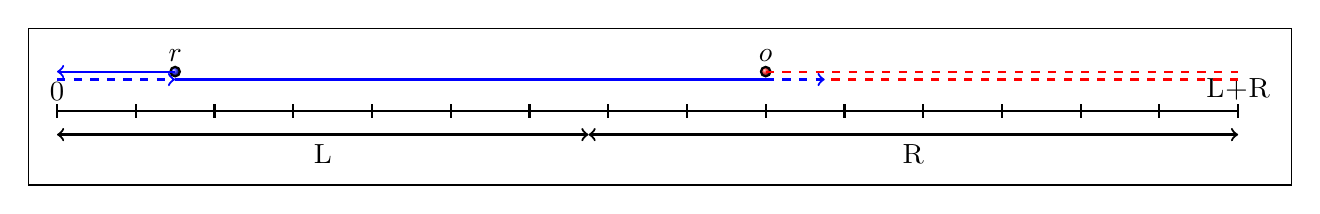
\begin{tikzpicture}[thick,framed]
%draw players
  \draw (0,0) -- (\len,0);
  \draw[snake=ticks,segment length=1cm] (0,0) -- (\len,0);
  \node[above] at (0,0) {$\textsc{0}$};% label the hinge
  \node[above] at (\len,0) {$\textsc{L+R}$};% label the hinge
  
  \filldraw[ball color=blue!80,shading=ball] (0.1*\len,0.5) circle
        (0.06cm) node[above]{\rob};% p1
  
  \filldraw[ball color=red!80,shading=ball] (0.6*\len,0.5) circle
        (0.06cm) node[above]{\opp};% p2
     
   % draw path
   \draw[->, blue] (0.1*\len,0.5) -- (0.0*\len,0.5)
	  	node[pos=0.7,above]{}; % path1 p2
    \draw[->, blue, dashed] (0.0*\len,0.4) -- (0.1*\len,0.4)
	  	node[pos=0.7,above]{}; % path1 p2
    \draw[-, blue] (0.1*\len,0.4) -- (0.6*\len,0.4)
	  	node[pos=0.7,above]{}; % path1 p2
    \draw[->, blue, dashed] (0.6*\len,0.4) -- (0.65*\len,0.4)
	  	node[pos=0.7,above]{}; % path1 p2
   
   \draw[-, red, dashed] (0.6*\len,0.5) -- (\len,0.5)
	  	node[pos=0.5,above]{}; % path1 p1
   \draw[-, red, dashed] (\len,0.4) -- (0.65*\len,0.4)
	  	node[pos=0.5,above]{}; % path1 p1
   
   % draw axis
   \draw[<->] (0, -0.3) -- (0.45*\len, -0.3)
        node[pos=0.5,below]{$\textsc{L}$}; % Left hand
   \draw[<->] (0.45*\len, -0.3) -- (\len, -0.3)
        node[pos=0.5,below]{$\textsc{R}$}; % Right Hand
\end{tikzpicture}
\caption{Case 4}
\end{figure}
  \underline{Happen When:} This case is similar to the first case. If \rob is meeting \opp before he reached its initial position again, then it should hold: $2(d-o)>r+o\Rightarrow 2d-3o-r>0$.

\underline{Profit:} It is simple to deduct the gained distance here: $\abs*{o}$.
}
\end{caseof}

In order to get a basic idea over which function is greater than the other, we will plot the two functions, over \opp values at range $[51,99]$ in world of size $100$. The functions looks as follows:

\begin{figure}[H]
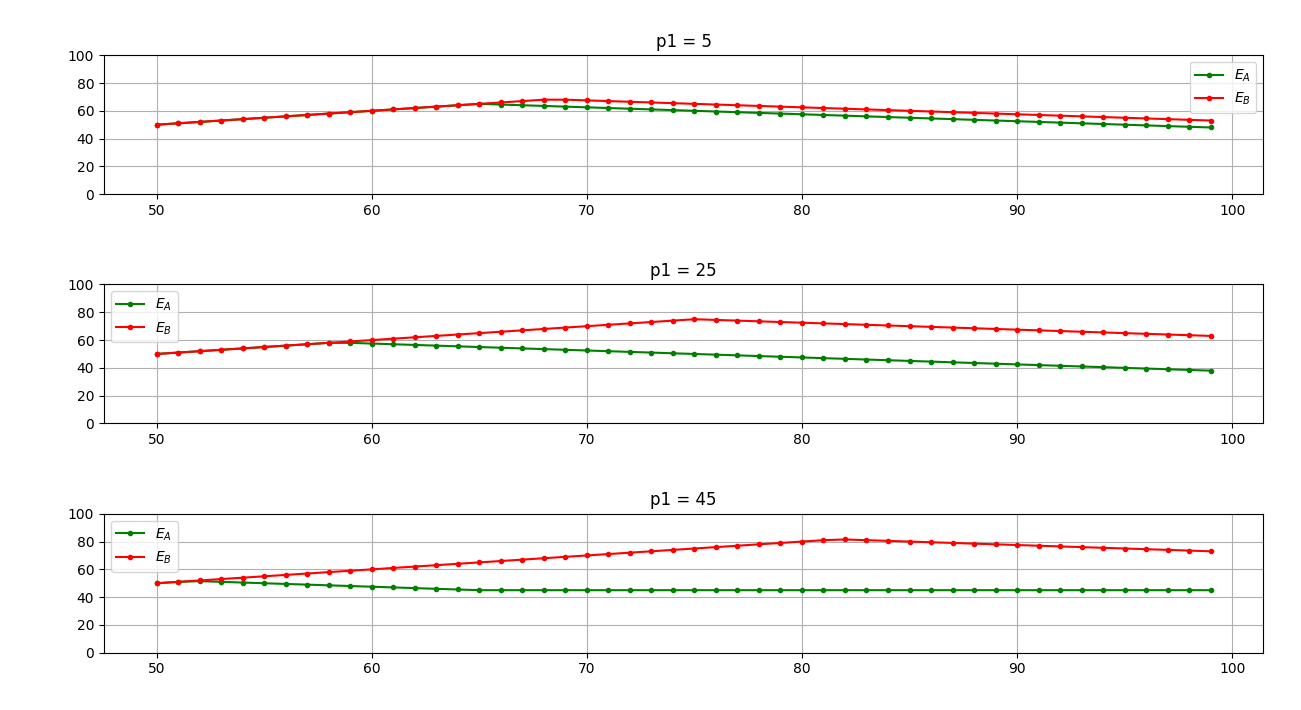
\includegraphics[width=\textwidth]{Images/GainedProfitp2SecondHalfWorld.png}
\caption{Expected profits for different cases of \rob}
\end{figure}

And as was expected, in all cases, it is indeed better for \rob to play $\gf$ instead of \gn. The proof for that is pretty simple: Consider each one of the 4 cases $E_\gn$ consists upon, and prove that each one of them holds $E_B \geq E_\gn$:
\begin{itemize}
\item Case 1: Since $E_\gn=r$, which is lower than both cases of $E_\gf$, it holds tat $E_B \geq E_\gn$.
\item Case 2: Take some $\left<d,r,o\right>$ that holds case 2 requirements. If this triplet hold $2d+r-3o$ then $E_\gf$ is in the first case, and we simply see that $E_B \geq E_\gn$. On the other hand, if it is not, and we fall in case 2, it simple to show that $E_B =\frac{2d-r-o}{2} > o = E_\gn$: since the triplet holds $E_\gn$ requirements, then $2d-3o-r<0\Rightarrow \frac{2d-3o-r}{2}<0\Rightarrow \frac{2d-o-r}{2}<o$, which concludes that proof for case 2.
\item Case 3: From $E_\gf$ condition, $d-o<r$, we get that $E_B=\frac{2d-o-r}{2}<\frac{d+r-r}{2}=\frac{d}{2}<o=E_\gn$, which proves that if $<d,r,o>$ holds $E_\gn$ second condition, and $E_\gf$ third condition, it holds that $E_B\geq E_\gn$. The first case is strait forward.
\item Case 4: Simply, if $2d-3o-r>0$, then of coarse $2d-3o+r>0$ since $r>0$. And also for case 4 it holds: $E_B \geq E_\gn$.
\end{itemize}

\end{proof}

\begin{theorem}
If \opp is playing \gn, the best thing \rob can do is going toward \opp position.
\end{theorem}
\begin{proof}
Follows directly from lemmas 4.5 to 4.7.
\end{proof}

\newpage

\subsection{Problems 3(Known strategy, unknown position)}\label{subsections: 1D, known strategy, hidden position}
In this part, we will consider the problems in which \opp initial position is unknown to us, and therefore we need to compute the expected profits, and the probabilities for them to occur.
\subsubsection{$S_{\opp}=\gn$}
\begin{caseof}
  \case{$ \opp \in \left(0,r\right),S_{\opp}=\gn$}
  {
  As the title above indicates, assume that \opp is playing strategy \gn, and that it is to the left of \rob. Initially, let us assume that $S_{\rob}=\gn$ We have two cases here:
First, if $o\in\left(0,\frac{2r}{3}\right)$, then in the time it takes \rob to go to 0 and then to its initial position, \opp managed to reach \opp initial position, therefore covering all the ground between them. After they will meet, \rob will turn and go to the far side, thus covering $d-r$ ground.
On the other hand, if $o\in\left(\frac{2r}{3},r\right)$, in the time it takes \rob to go to 0 and then to its initial position, \opp still has ground to cover. After moving $2o$ steps to the left, it moves for $\frac{r-3o}{2}$, meeting \rob, and then turning around and going for $d-r$ steps.
Note that for the first case to happen, \opp needs to 'fall' at most in two-third of \rob, and since we know that $o\in\left(0,r\right)$, then $P\left(o\in\left(0,\frac{2r}{3}\right)\right) = \frac{2}{3}$. In the same way, we get that $P\left(o\in\left(\frac{2r}{3},r\right)\right) = \frac{1}{3}$.
We combine the two cases, and we get that:

\begin{equation}
\underset{S_{\rob}=\gn,S_{\opp}=\gn}{E_{r}}=\abs*{(d-r)+\frac{1}{3}\left(2o+\frac{r-3o}{2}\right) + \frac{2}{3}\left(r-o\right)}
\end{equation}

Now, let us assume that $S_{\rob}=\gn$. This means that \rob is moving right, and away from \opp. Since $o < r < \frac{d}{2}$, \rob will cover all the way to $d$, and then turns around and go over already covered until meeting \opp. Therefore, the expected profit is:

\begin{equation}
\underset{S_{\rob}=\gf,S_{\rob}=\gn}{E_{r}}=\abs*{d-r}
\end{equation}

\textbf{Probability:} The probability for the this case to happen is: $\frac{r}{2}$.
  }
  \case{$ \opp \in\left(r,\frac{d}{2}\right),S_{\opp}=\gn$}
  {
  First, let us assume that $S_{\rob}=\gn$. The two players go the same way until \rob turns around and they meet. According to the computation done in Lemma 4.6, the expected profit is:
\begin{equation}
\underset{S_{\rob}=\gn,S_{\rob}=\gn}{E_{r}}= \abs*{r+\max\left(\frac{o-3r}{2},0\right)}
\end{equation}

Now, let us assume that $S_{\rob}=\gn$. The two players go toward each other, and this expected profit is easy to compute:
\begin{equation}
\underset{S_{\rob}=\gf,S_{\rob}=\gn}{E_{r}}= \abs*{\frac{o-r}{2}+r}=\abs*{\frac{o+r}{2}}
\end{equation}

\textbf{Probability:} The probability for the this case to happen is: $\frac{\frac{d}{2}-r}{2}$.
  }
  \case{$ \opp \in\left(\frac{d}{2},d\right),S_{\opp}=\gn$}
  {According to lemma 4.7, we know the gained profits for this case, and they are as follows:
\[f_\gn(x)=\begin{cases}
r+\frac{2d-r-o}{2},&2d+r-3o<0\\
p2,&2d+r-3o>0\\
\end{cases}\]

The probability for the first case is: 
\[P(2d+r-3o>0)=P\left(o<\frac{2d+r}{3}\right)=\frac{\int_0^{\frac{d}{2}}\frac{2d+r}{3}-\frac{d}{2}\,dr}{\frac{d^2}{4}}=\frac{\frac{2d}{3}\cdot \frac{d}{2}-\frac{d}{2}\cdot\frac{d}{2}+\frac{d^2}{12}}{\frac{d^2}{4}}=\frac{\frac{d^2}{8}}{\frac{d^2}{4}}=\frac{1}{2}\] and hence: $P\left(2d+r-3p-2<0\right)=\frac{1}{2}$.

\[f_\gf(x)=\begin{cases}
p1,&2d-3r-o<0\\
\frac{2d-r-o}{2},&2d-3o-r<0 \textsc{ and } r<d-o\\
\frac{2d-r-o}{2},&2d-3r-o>0 \textsc{ and } r>d-o\\
p2,&2d-3o-p1>0\\
\end{cases}\]

\textbf{Probability:}
For the first case, we would like to find the probability $P\left(2d-3ro<0\right)=P\left(o>2d-3r\right)$. Notice that for $0<r<\frac{d}{3}$, it holds $2d-3r>d$, and since $o<d$, $\nexists o s.t. 2d-3r<o$. And when $\frac{d}{3}<r<\frac{d}{2}$, it holds $2d-3r<d$, thus \opp has $d-\left(2d-3r\right)$ area to fall into. 
Therefore, the total probability is:
\[P\left(2d-3r-o<0\right)=\frac{\int_{\frac{d}{3}}^{\frac{d}{2}}3x-d\, dx}{\frac{d^2}{4}}=\frac{\left[\frac{3x^2}{2}-d\cdot x\right]_{\frac{d}{3}}^{\frac{d}{2}}}{\frac{d^2}{4}}=\frac{\frac{d^2}{24}}{\frac{d^2}{4}}=\frac{1}{6}\]

For the third case, we would like to find the probability of $2d-3r-o>0$ and $r>d-o$. Let us distinct between two different cases - when $0 < r<\frac{d}{3}$ and when $\frac{d}{3} < r < \frac{d}{2}$.
\begin{itemize}
\item If we are talking about the first case, then it holds $2d-3r>o$ for all \opp, and we should find when the second condition happen. Notice that for some $r=\epsilon$, \opp needs to fall in the range $\left[d-\epsilon,d\right]$.
\item When considering the second case, it holds  that $\frac{d}{2}<2d-3r<d$. Since as in the previous case \opp must hold $o>d-r$. Consider some $r=\epsilon$. \opp can fall only in the range $\left[d-\epsilon,2d-3\epsilon\right]$ (notice that indeed $\frac{d}{2}<d-\epsilon < 2d-3\epsilon < d$), which is area of size $2d-3\epsilon - (d-\epsilon)=d-2\epsilon$.
\end{itemize}

Let us compute the total probability:
\[P(2d-3r-o>0\textsf{ and }r>d-o)=\frac{\int_{0}^{\frac{d}{3}}x\,dx+\int_{\frac{d}{3}}^{\frac{d}{2}}d-2x\,dx}{\frac{d^2}{4}}=\frac{\left[\frac{x^2}{2}\right]_{}^{\frac{d}{3}}+\left[dx-x^2\right]_{\frac{d}{3}}^{\frac{d}{2}}}{\frac{d^2}{4}}=\frac{\frac{d^2}{18}+\frac{d^2}{36}}{\frac{d^2}{4}}=\frac{1}{3}\]

For the forth case, we would like to find $P\left(2d-3o-r>0\right)=P\left(\frac{2d-r}{3}>o\right)$. It holds that $\forall r\in\left[0,\frac{d}{2}\right]$ the case holds, and therefore \opp has $\frac{2d-r}{3}-\frac{d}{2}$ area to fall into. Hence, the probability is:
\[P\left(2d-3o-r>0\right)=\frac{\int_{0}^{\frac{d}{2}}\frac{2d-x}{3}-\frac{d}{2}\,dx}{\frac{d^2}{4}}=\frac{\left[\frac{2d\cdot x}{3}-\frac{x^2}{6}-\frac{d\cdot x}{2}\right]_{0}^{\frac{d}{2}}}{\frac{d^2}{4}}=\frac{\frac{2d}{3}\cdot\frac{d}{2}-\frac{d^2}{24}-\frac{d^2}{4}}{\frac{d^2}{4}}=\frac{\frac{d^2}{24}}{\frac{d^2}{4}}=\frac{1}{6}\]

And the second case is what left, and so its probability is $\frac{1}{3}$.
  }
\end{caseof}

\case{Putting it all together}
{Let us put together all of the above; The total expected profit consists of all the gained profit for each case, multiplied by its probability. We will have two such values, one for when $S_{\rob}=\gn$, and one for when $S_{\rob}=\gn$.

Let us define $f_\gn$ and $P_\gn$, where $f_\gn$ stands for profit function, depends in \opp position on the world, and $P_\gn$ is the probability for the specific \opp value, as follows:
\[f_\gn\left(x\right)=\begin{cases}
\abs*{(d-r)+\frac{1}{3}\left(2x+\frac{r-3x}{2}\right) + \frac{2}{3}\left(r-o\right)},&0<x<r\\
\abs*{r+\max\left(\frac{x-3r}{2},0\right)}
,&r<x<\frac{d}{2}\\
r,&\frac{d}{2}<x<d \textsf{ and } 2d-3r-o<0\\
\frac{2d-r-x}{2},&\frac{d}{2}<x<d \textsf{ and } 2d-3x-r<0 \textsf{ and } r < d-x\\
\frac{2d-r-x}{2},&\frac{d}{2}<x<d \textsf{ and } 2d-3r-x>0 \textsf{ and } r>d-x\\
x,&\frac{d}{2}<x<d \textsf{ and } 2d-3x-r>0\\
\end{cases}\]

\[P_\gn\left(x\right)=\begin{cases}
\frac{r}{d},&0<x<r\\
\frac{\frac{d}{2}-r}{d},&r<x<\frac{d}{2}\\
\frac{1}{2}\cdot \frac{1}{6},&\frac{d}{2}<x<d \textsf{ and } 2d-3r-o<0\\
\frac{1}{2}\cdot \frac{1}{3},&\frac{d}{2}<x<d \textsf{ and } 2d-3x-r<0 \textsf{ and } r < d-x\\
\frac{1}{2}\cdot \frac{1}{3},&\frac{d}{2}<x<d \textsf{ and } 2d-3r-x>0 \textsf{ and } r>d-x\\
\frac{1}{2}\cdot \frac{1}{6},&\frac{d}{2}<x<d \textsf{ and } 2d-3x-r>0\\
\end{cases}\]

\begin{equation}
E_{S_{\rob}=\gn,S_{\rob}=\gn}=\frac{\sum_{o=0}^{d}{f_{A}\left(o\right)\cdot P_{A}\left(o\right)}}{d}
\end{equation}

In a similar way, let us define the functions $f_\gf$ and $P_\gf$:

\[f_\gf\left(x\right)=\begin{cases}
\abs*{d-r},&0<x<r\\
\abs*{\frac{x+r}{2}},&r<x<\frac{d}{2}\\
r+\frac{2d-r-x}{2},&\frac{d}{2}<x<d \textsf{ and } 2d+r-3x<0\\
x,&\frac{d}{2}<x<d \textsf{ and } 2d+r-3x>0\\
\end{cases}\]

\[P_\gf\left(x\right)=\begin{cases}
\frac{r}{d},&0<x<r\\
\frac{\frac{d}{2}-r}{d},&r<x<\frac{d}{2}\\
\frac{1}{2}\cdot \frac{1}{2},&\frac{d}{2}<x<d \textsf{ and } 2d+r-3x<0\\
\frac{1}{2}\cdot \frac{1}{2},&\frac{d}{2}<x<d \textsf{ and } 2d+r-3x>0\\
\end{cases}\]

\begin{equation}
E_{S_{\rob}=\gf,S_{\rob}=\gn}=\frac{\sum_{o=0}^{d}{f_{B}\left(o\right)\cdot P_{B}\left(o\right)}}{d}
\end{equation}

\textbf{Plotting:} In order to get a general idea of the functions, we plotted the expected profits. The results that shown in Figure something, clearly indicate that if one have no information over its opponent's position, it should choose playing $\gf$.

\begin{figure}[H]
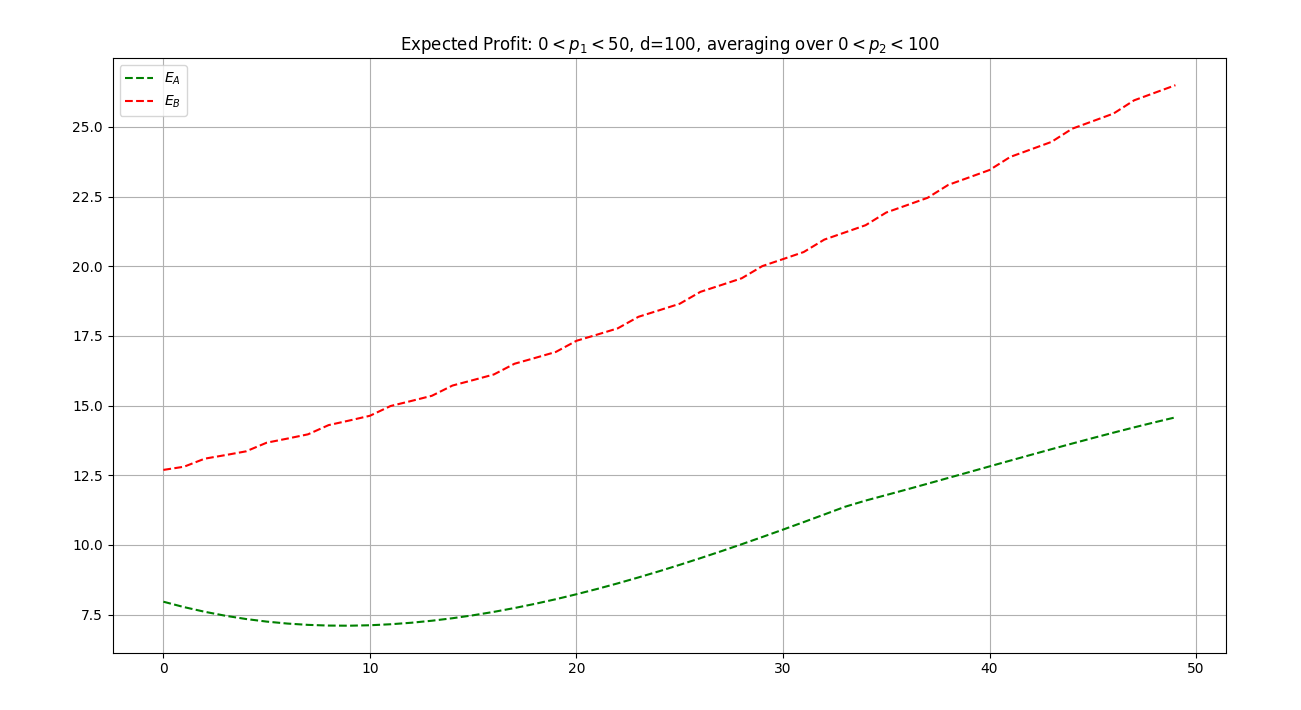
\includegraphics[width=\textwidth]{Images/E1_E2_p2A_abs.png}
\caption{Utility functions, $i_{\rob}$ values vs. Expected profits, for $0<i_{\opp}<100$}
\end{figure}}
\subsubsection{$S_{\opp}=\gf$}
As the title indicates, throughout this section assume the $S_{\opp}=\gf$. Let us compute the profit and probability for each case of \opp initial position, and use that to compute the total expected profit for this section.
\begin{caseof}
  \case{$ \opp \in\left(0,r\right)$}
  {
  
\begin{figure}[H]
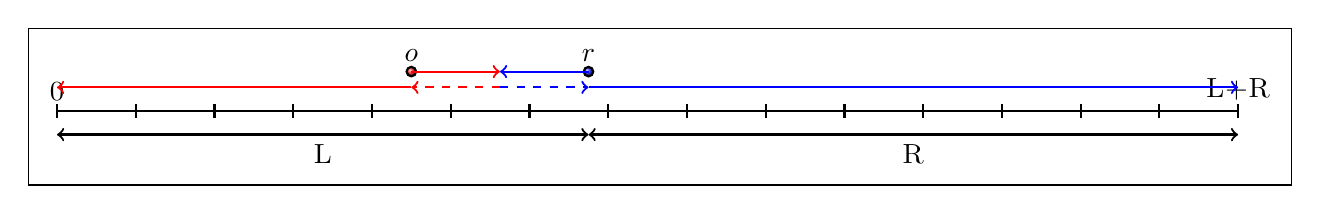
\begin{tikzpicture}[thick,framed]
%draw players
  \draw (0,0) -- (\len,0);
  \draw[snake=ticks,segment length=1cm] (0,0) -- (\len,0);
  \node[above] at (0,0) {$\textsc{0}$};% label the hinge
  \node[above] at (\len,0) {$\textsc{L+R}$};% label the hinge
  
  \filldraw[ball color=blue!80,shading=ball] (0.45*\len,0.5) circle
        (0.06cm) node[above]{\rob};% p1
  
  \filldraw[ball color=red!80,shading=ball] (0.3*\len,0.5) circle
        (0.06cm) node[above]{\opp};% p2
     
   % draw path
   \draw[->, blue] (0.45*\len,0.5) -- (0.375*\len,0.5)
	  	node[pos=0.7,above]{}; % path1 p2 
   \draw[->, blue, dashed] (0.375*\len,0.3) -- (0.45*\len,0.3)
	  	node[pos=0.7,above]{}; % path1 p2  
   \draw[->, blue] (0.45*\len,0.3) -- (\len,0.3)
	  	node[pos=0.7,above]{}; % path1 p2 
   
   \draw[->, red] (0.3*\len,0.5) -- (0.375*\len,0.5)
	  	node[pos=0.5,above]{}; % path1 p1
   \draw[->, red, dashed] (0.375*\len,0.3) -- (0.3*\len,0.3)
	  	node[pos=0.5,above]{}; % path1 p1
   \draw[->, red] (0.3*\len,0.3) -- (0.0*\len,0.3)
	  	node[pos=0.5,above]{}; % path1 p1
   
        
   % draw axis
   \draw[<->] (0, -0.3) -- (0.45*\len, -0.3)
        node[pos=0.5,below]{$\textsc{L}$}; % Left hand
   \draw[<->] (0.45*\len, -0.3) -- (\len, -0.3)
        node[pos=0.5,below]{$\textsc{R}$}; % Right Hand
\end{tikzpicture}
\caption{$S_{\rob}=\gn$}
\end{figure}

Figure1 is simple: both players start by going toward each other, then meet. They turn around, and do until reaching the far edge. The profits are:
\[E_{S_{\rob}=\gn,S_{\opp}=\gf}=\abs*{\frac{r-o}{2}+(d-r)}=\abs*{\frac{2d-3r-o}{2}}\]
 
On the other hand, in Figure 2 we see the case when $S_{\rob}=\gn$, and both players start by going right. From their initial position we know that after \rob reached the far edge, it turns, and he meet \opp over covered ground.

\begin{figure}[H]
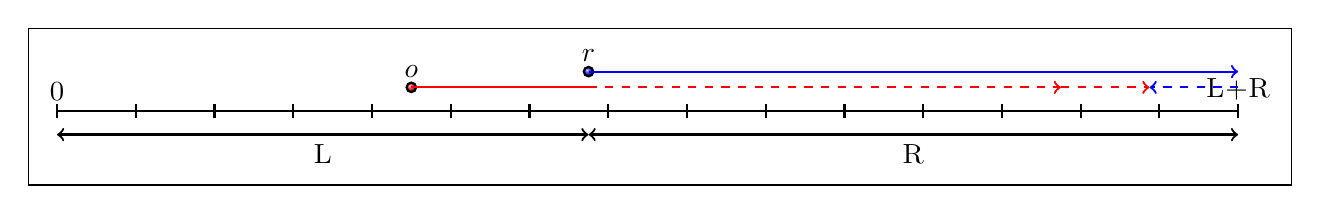
\begin{tikzpicture}[thick,framed]
%draw players
  \draw (0,0) -- (\len,0);
  \draw[snake=ticks,segment length=1cm] (0,0) -- (\len,0);
  \node[above] at (0,0) {$\textsc{0}$};% label the hinge
  \node[above] at (\len,0) {$\textsc{L+R}$};% label the hinge
  
  \filldraw[ball color=blue!80,shading=ball] (0.45*\len,0.5) circle
        (0.06cm) node[above]{\rob};% p1
  
  \filldraw[ball color=red!80,shading=ball] (0.3*\len,0.3) circle
        (0.06cm) node[above]{\opp};% p2
     
   % draw path
   \draw[->, blue] (0.45*\len,0.5) -- (\len,0.5)
	  	node[pos=0.7,above]{}; % path1 p2
   \draw[->, blue, dashed] (\len,0.3) -- (0.925*\len,0.3)
	  	node[pos=0.7,above]{}; % path1 p2 
   
   \draw[-, red] (0.3*\len,0.3) -- (0.45*\len,0.3)
	  	node[pos=0.5,above]{}; % path1 p1
   \draw[->, red, dashed] (0.45*\len,0.3) -- (0.85*\len,0.3)
	  	node[pos=0.5,above]{}; % path1 p1
   \draw[->, red, dashed] (0.85*\len,0.3) -- (0.925*\len,0.3)
	  	node[pos=0.5,above]{}; % path1 p1
   
   
        
   % draw axis
   \draw[<->] (0, -0.3) -- (0.45*\len, -0.3)
        node[pos=0.5,below]{$\textsc{L}$}; % Left hand
   \draw[<->] (0.45*\len, -0.3) -- (\len, -0.3)
        node[pos=0.5,below]{$\textsc{R}$}; % Right Hand
\end{tikzpicture}
\caption{$S_{\rob}=\gn$}
\end{figure}

The profit is:

\[E_{S_{\rob}=\gf,S_{\opp}=\gf}=\abs*{d-r}\]

\textbf{Probability:}
The probability for this case is $\frac{r}{d}$, which is the cumulative distribution of \opp position function. That is \rob can appear on all the range that \rob  is setting.
}

\case{$ \opp \in\left(r,\frac{d}{2}\right)$}
{

\begin{figure}[H]
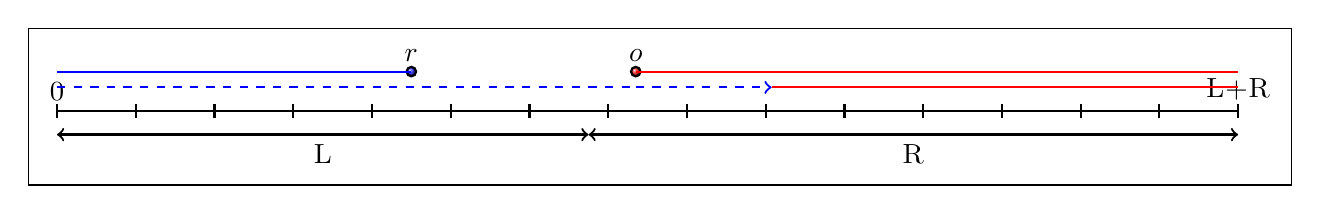
\begin{tikzpicture}[thick,framed]
%draw players
  \draw (0,0) -- (\len,0);
  \draw[snake=ticks,segment length=1cm] (0,0) -- (\len,0);
  \node[above] at (0,0) {$\textsc{0}$};% label the hinge
  \node[above] at (\len,0) {$\textsc{L+R}$};% label the hinge
  
  \filldraw[ball color=blue!80,shading=ball] (0.3*\len,0.5) circle
        (0.06cm) node[above]{\rob};% p1
  
  \filldraw[ball color=red!80,shading=ball] (0.49*\len,0.5) circle
        (0.06cm) node[above]{\opp};% p2
     
   % draw path
   \draw[-, blue] (0.3*\len,0.5) -- (0.0*\len,0.5)
	  	node[pos=0.7,above]{}; % path1 p2
   \draw[-, blue,dashed] (0.0*\len,0.3) -- (0.49*\len,0.3)
	  	node[pos=0.7,above]{}; % path1 p2
   \draw[->, blue,dashed] (0.49*\len,0.3) -- (0.605*\len,0.3)
	  	node[pos=0.7,above]{}; % path1 p2
   
   
   \draw[-, red] (0.49*\len,0.5) -- (\len,0.5)
	  	node[pos=0.5,above]{}; % path1 p1
   \draw[-, red] (\len,0.3) -- (0.605*\len,0.3)
	  	node[pos=0.5,above]{}; % path1 p1
  
   
   % draw axis
   \draw[<->] (0, -0.3) -- (0.45*\len, -0.3)
        node[pos=0.5,below]{$\textsc{L}$}; % Left hand
   \draw[<->] (0.45*\len, -0.3) -- (\len, -0.3)
        node[pos=0.5,below]{$\textsc{R}$}; % Right Hand
\end{tikzpicture}
\caption{$S_{\rob}=\gn$}
\end{figure}

The first case is the more interesting one: The distance \rob covers from its initial position, to the near edge, and then to \opp initial position is: $r+o$, which is less than what \opp needs to cover only in order to reach its initial position: $2(d-o)$. because both $r<\frac{d}{2}$ and $o<\frac{d}{2}$, then of coarse: $r+o<d<2(d-o)$.
Therefore, the gained profit here is:

\[E_{S_{\rob}=\gn,S_{\opp}=\gf}=\abs*{o}\]


\begin{figure}[H]
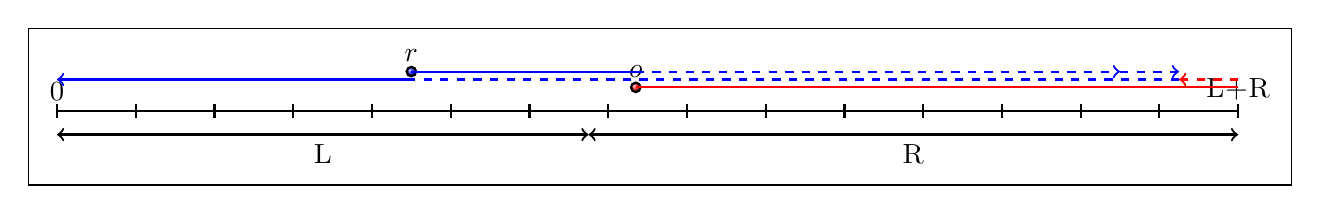
\begin{tikzpicture}[thick,framed]
%draw players
  \draw (0,0) -- (\len,0);
  \draw[snake=ticks,segment length=1cm] (0,0) -- (\len,0);
  \node[above] at (0,0) {$\textsc{0}$};% label the hinge
  \node[above] at (\len,0) {$\textsc{L+R}$};% label the hinge
  
  \filldraw[ball color=blue!80,shading=ball] (0.3*\len,0.5) circle
        (0.06cm) node[above]{\rob};% p1
  
  \filldraw[ball color=red!80,shading=ball] (0.49*\len,0.3) circle
        (0.06cm) node[above]{\opp};% p2
     
   % draw path
   \draw[-, blue] (0.3*\len,0.5) -- (0.49*\len,0.5)
	  	node[pos=0.7,above]{}; % path1 p2
   \draw[->, blue, dashed] (0.49*\len,0.5) -- (0.9*\len,0.5)
	  	node[pos=0.7,above]{}; % path1 p2
   \draw[->, blue, dashed] (0.9*\len,0.5) -- (0.95*\len,0.5)
	  	node[pos=0.7,above]{}; % path1 p2
   \draw[-, blue, dashed] (0.95*\len,0.4) -- (0.3*\len,0.4)
	  	node[pos=0.7,above]{}; % path1 p2 
   \draw[->, blue] (0.3*\len,0.4) -- (0.0*\len,0.4)
	  	node[pos=0.7,above]{}; % path1 p2 
   
   \draw[-, red] (0.49*\len,0.3) -- (\len,0.3)
	  	node[pos=0.5,above]{}; % path1 p1
   \draw[->, red, dashed] (\len,0.4) -- (0.95*\len,0.4)
	  	node[pos=0.5,above]{}; % path1 p1
   
   
        
   % draw axis
   \draw[<->] (0, -0.3) -- (0.45*\len, -0.3)
        node[pos=0.5,below]{$\textsc{L}$}; % Left hand
   \draw[<->] (0.45*\len, -0.3) -- (\len, -0.3)
        node[pos=0.5,below]{$\textsc{R}$}; % Right Hand
\end{tikzpicture}
\caption{$S_{\rob}=\gn$}
\end{figure}

In Figure 4, $o\in\left(r,\frac{d}{2}\right)$. The profit for this case, as one can see, is:

\[E_{S_{\rob}=\gf,S_{\opp}=\gf}=\abs*{(o-r)+r}=\abs*{o}\]

\textbf{Probability:} As before, we take the cumulative distribution, so the probability is: $\frac{\frac{d}{2}-r}{d}$.

}

\case{$ \opp \in\left(\frac{d}{2},d\right)$}
{

First, consider $S_{\rob}=\gn$. We have two sub-cases; In the first, \rob manage to go to the near edge and back, and also to cover new ground, before meeting \opp. And in the second, it does not. The first case happen only when $o-2r>r\Rightarrow 3r<o$, and vice versa.

\begin{figure}[H]
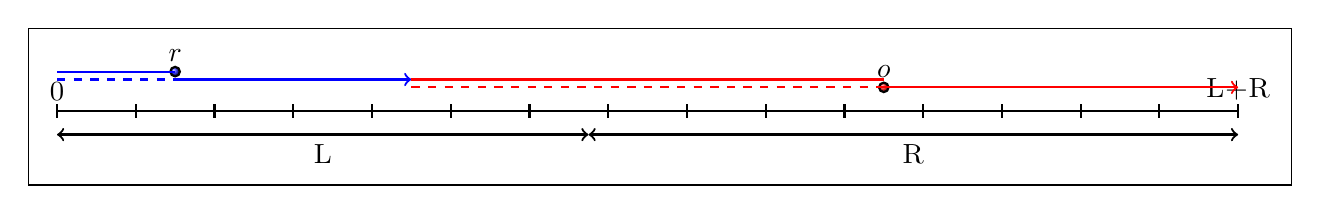
\begin{tikzpicture}[thick,framed]
%draw players
  \draw (0,0) -- (\len,0);
  \draw[snake=ticks,segment length=1cm] (0,0) -- (\len,0);
  \node[above] at (0,0) {$\textsc{0}$};% label the hinge
  \node[above] at (\len,0) {$\textsc{L+R}$};% label the hinge
  
  \filldraw[ball color=blue!80,shading=ball] (0.1*\len,0.5) circle
        (0.06cm) node[above]{\rob};% p1
  
  \filldraw[ball color=red!80,shading=ball] (0.7*\len,0.3) circle
        (0.06cm) node[above]{\opp};% p2
     
   % draw path
   \draw[-, blue] (0.1*\len,0.5) -- (0.0*\len,0.5)
	  	node[pos=0.7,above]{}; % path1 p2
   \draw[-, blue,dashed] (0.0*\len,0.4) -- (0.1*\len,0.4)
	  	node[pos=0.7,above]{}; % path1 p2
   \draw[->, blue] (0.1*\len,0.4) -- (0.3*\len,0.4)
	  	node[pos=0.7,above]{}; % path1 p2
   
   \draw[-, red] (0.7*\len,0.4) -- (0.5*\len,0.4)
	  	node[pos=0.5,above]{}; % path1 p1
   \draw[-, red] (0.5*\len,0.4) -- (0.3*\len,0.4)
	  	node[pos=0.5,above]{}; % path1 p1
   \draw[-, red, dashed] (0.3*\len,0.3) -- (0.7*\len,0.3)
	  	node[pos=0.5,above]{}; % path1 p1
   \draw[->, red] (0.7*\len,0.3) -- (\len,0.3)
	  	node[pos=0.5,above]{}; % path1 p1
   
   
        
   % draw axis
   \draw[<->] (0, -0.3) -- (0.45*\len, -0.3)
        node[pos=0.5,below]{$\textsc{L}$}; % Left hand
   \draw[<->] (0.45*\len, -0.3) -- (\len, -0.3)
        node[pos=0.5,below]{$\textsc{R}$}; % Right Hand
\end{tikzpicture}
\caption{$S_{\rob}=\gn, 3r<o$}
\end{figure}

The first case is described in Figure 5. The distance \rob is doing after reaching its initial position again is: $\frac{o-2r-r}{2}=\frac{o-3r}{2}$.
Therefore, the gained profit is:
\[E_{S_{\rob}=\gn,S_{\opp}=\gf}=\abs*{r+\frac{o-3r}{2}}\]




\begin{figure}[H]
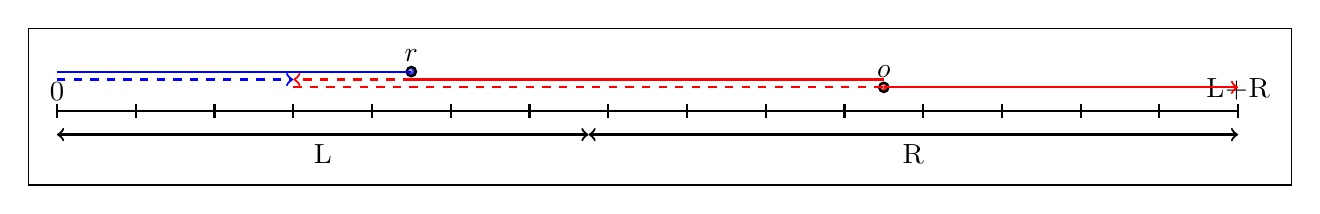
\begin{tikzpicture}[thick,framed]
%draw players
  \draw (0,0) -- (\len,0);
  \draw[snake=ticks,segment length=1cm] (0,0) -- (\len,0);
  \node[above] at (0,0) {$\textsc{0}$};% label the hinge
  \node[above] at (\len,0) {$\textsc{L+R}$};% label the hinge
  
  \filldraw[ball color=blue!80,shading=ball] (0.3*\len,0.5) circle
        (0.06cm) node[above]{\rob};% p1
  
  \filldraw[ball color=red!80,shading=ball] (0.7*\len,0.3) circle
        (0.06cm) node[above]{\opp};% p2
     
   % draw path
   \draw[-, blue] (0.3*\len,0.5) -- (0.0*\len,0.5)
	  	node[pos=0.7,above]{}; % path1 p2 
   \draw[->, blue, dashed] (0.0*\len,0.4) -- (0.2*\len,0.4)
	  	node[pos=0.7,above]{}; % path1 p2 
   
   \draw[-, red] (0.7*\len,0.4) -- (0.4*\len,0.4)
	  	node[pos=0.5,above]{}; % path1 p1
   \draw[-, red] (0.4*\len,0.4) -- (0.3*\len,0.4)
	  	node[pos=0.5,above]{}; % path1 p1
   \draw[->, red, dashed] (0.3*\len,0.4) -- (0.2*\len,0.4)
	  	node[pos=0.5,above]{}; % path1 p1
   \draw[-, red, dashed] (0.2*\len,0.3) -- (0.7*\len,0.3)
	  	node[pos=0.5,above]{}; % path1 p1
   \draw[->, red] (0.7*\len,0.3) -- (\len,0.3)
	  	node[pos=0.5,above]{}; % path1 p1
   
        
   % draw axis
   \draw[<->] (0, -0.3) -- (0.45*\len, -0.3)
        node[pos=0.5,below]{$\textsc{L}$}; % Left hand
   \draw[<->] (0.45*\len, -0.3) -- (\len, -0.3)
        node[pos=0.5,below]{$\textsc{R}$}; % Right Hand
\end{tikzpicture}
\caption{$S_{\rob}=\gn, 3r>o$}
\end{figure}

The second sub-case is described in Figure 6. The profit is:
\[E_{S_{\rob}=\gn,S_{\opp}=\gf}=\abs*{r}\]


On the other, consider the case when $S_{\rob}=\gn$. The case is described in Figure 7.

\begin{figure}[H]
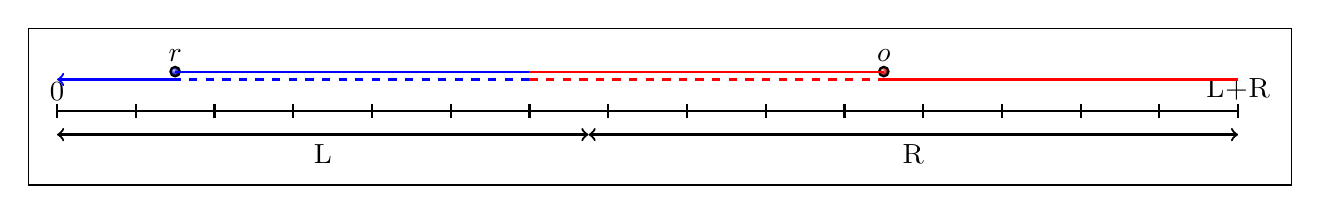
\begin{tikzpicture}[thick,framed]
%draw players
  \draw (0,0) -- (\len,0);
  \draw[snake=ticks,segment length=1cm] (0,0) -- (\len,0);
  \node[above] at (0,0) {$\textsc{0}$};% label the hinge
  \node[above] at (\len,0) {$\textsc{L+R}$};% label the hinge
  
  \filldraw[ball color=blue!80,shading=ball] (0.1*\len,0.5) circle
        (0.06cm) node[above]{\rob};% p1
  
  \filldraw[ball color=red!80,shading=ball] (0.7*\len,0.5) circle
        (0.06cm) node[above]{\opp};% p2
     
   % draw path
   \draw[-, blue] (0.1*\len,0.5) -- (0.4*\len,0.5)
	  	node[pos=0.7,above]{}; % path1 p2
   \draw[-, blue, dashed] (0.4*\len,0.4) -- (0.1*\len,0.4)
	  	node[pos=0.7,above]{}; % path1 p2
   \draw[->, blue] (0.1*\len,0.4) -- (0.0*\len,0.4)
	  	node[pos=0.7,above]{}; % path1 p2
   
   \draw[-, red] (0.7*\len,0.5) -- (0.4*\len,0.5)
	  	node[pos=0.5,above]{}; % path1 p1
   \draw[-, red, dashed] (0.4*\len,0.4) -- (0.7*\len,0.4)
	  	node[pos=0.5,above]{}; % path1 p1
   \draw[-, red] (0.7*\len,0.4) -- (\len,0.4)
	  	node[pos=0.5,above]{}; % path1 p1   
   
        
   % draw axis
   \draw[<->] (0, -0.3) -- (0.45*\len, -0.3)
        node[pos=0.5,below]{$\textsc{L}$}; % Left hand
   \draw[<->] (0.45*\len, -0.3) -- (\len, -0.3)
        node[pos=0.5,below]{$\textsc{R}$}; % Right Hand
\end{tikzpicture}
\caption{$S_{\rob}=\gn$}
\end{figure}

The expected profit is simple to compute:
\[E_{S_{\rob}=\gf,S_{\opp}=\gf}=\abs*{\frac{o-r}{2}+r}\]

\textbf{Probability:} As mentioned before, the first case happen only when $3r<o$, and the second case happen when $r>\frac{o}{3}$. Let us compute the probability of the second case: if $0<r<\frac{d}{6}$, then $2r<\frac{d}{2}$, and \opp has no 'land' to fall upon.
If $\frac{d}{6}<r<\frac{d}{3}$, \opp can fall in $3r-\frac{d}{2}$. And of course, if $\frac{d}{3}<r<\frac{d}{2}$, \rob has exactly $\frac{d}{2}$ area to fall in. We can summarize and get:

\[P\left(\frac{d}{2}<o<3r\right)=\frac{\int_{0}^{\frac{d}{6}} 0 \,dx + \int_{\frac{d}{6}}^{\frac{d}{3}} 3x-\frac{d}{2} \,dx + \int_{\frac{d}{3}}^{\frac{d}{2}} \frac{d}{2} \,dx}{\frac{d^2}{4}}=\frac{\left[\frac{3x^2}{2}-\frac{d}{2}\cdot x\right]_{\frac{d}{3}}^{\frac{d}{6}} + \left[\frac{d}{2}\cdot x\cdot x\right]_{\frac{d}{2}}^{\frac{d}{3}}}{\frac{d^2}{4}}=\frac{1}{2}\].

And, the probability for the first case, is \[P\left(o>r\right)=\frac{1}{2}\]
The probability for the total case is the cumulative distribution over half the world: $\frac{1}{2}$.
}

\case{Putting it all together}
{
Let us put together all of the above; The total expected profit consists of all the gained profit for each case, multiplied by its probability. We will have two such values, one for when $S_{\rob}=\gn$, and one for when $S_{\rob}=\gn$.

Let us define $f_\gn$ and $P_\gn$, where $f_\gn$ stands for profit function, depends in \opp position on the world, and $P_\gn$ is the probability for the specific \opp value, as follows:
\[f_\gn\left(x\right)=\begin{cases}
\abs*{\frac{r-x}{2}+(d-r)},&0<x<r\\
\abs*{x},&r<x<\frac{d}{2}\\
\abs*{r+\frac{o-3r}{2}},&\frac{d}{2}<x<d \textsf{ and } x>3r\\
\abs*{r},&\frac{d}{2}<x<d \textsf{ and } x<3r\\
\end{cases}\]

\[P_\gn\left(x\right)=\begin{cases}
\frac{r}{d},&0<x<r\\
\frac{\frac{d}{2}-r}{d},&r<x<\frac{d}{2}\\
\frac{1}{2}\cdot\frac{1}{2},&\frac{d}{2}<x<d \textsf{ and } x>3r\\
\frac{1}{2}\cdot\frac{1}{2},&\frac{d}{2}<x<d \textsf{ and } x<3r\\
\end{cases}\]

\begin{equation}
E_{S_{\rob}=\gn,S_{\opp}=\gf}=\frac{\sum_{o=0}^{d}{f_{A}\left(o\right)\cdot P_{A}\left(o\right)}}{d}
\end{equation}

In a similar way, let us define $f_\gf$ and $P_\gf$ as follows:
\[f_\gf\left(x\right)=\begin{cases}
\abs*{d-r},&0<x<r\\
\abs*{x},&r<x<\frac{d}{2}\\
\abs*{\frac{o-r}{2}+r},&\frac{d}{2}<x<d
\end{cases}\]

\[P_\gf\left(x\right)=\begin{cases}
\frac{r}{d},&0<x<r\\
\frac{\frac{d}{2}-r}{d},&r<x<\frac{d}{2}\\
\frac{1}{2},&\frac{d}{2}<x<d
\end{cases}\]

\begin{equation}
E_{S_{\rob}=\gf,S_{\opp}=\gf}=\frac{\sum_{o=0}^{d}{f_\gf\left(o\right)\cdot P_\gf\left(o\right)}}{d}
\end{equation}

\textbf{Plotting: } In order to get a general idea of how these functions looks like, we plotted them, one against the other player.
\begin{figure}
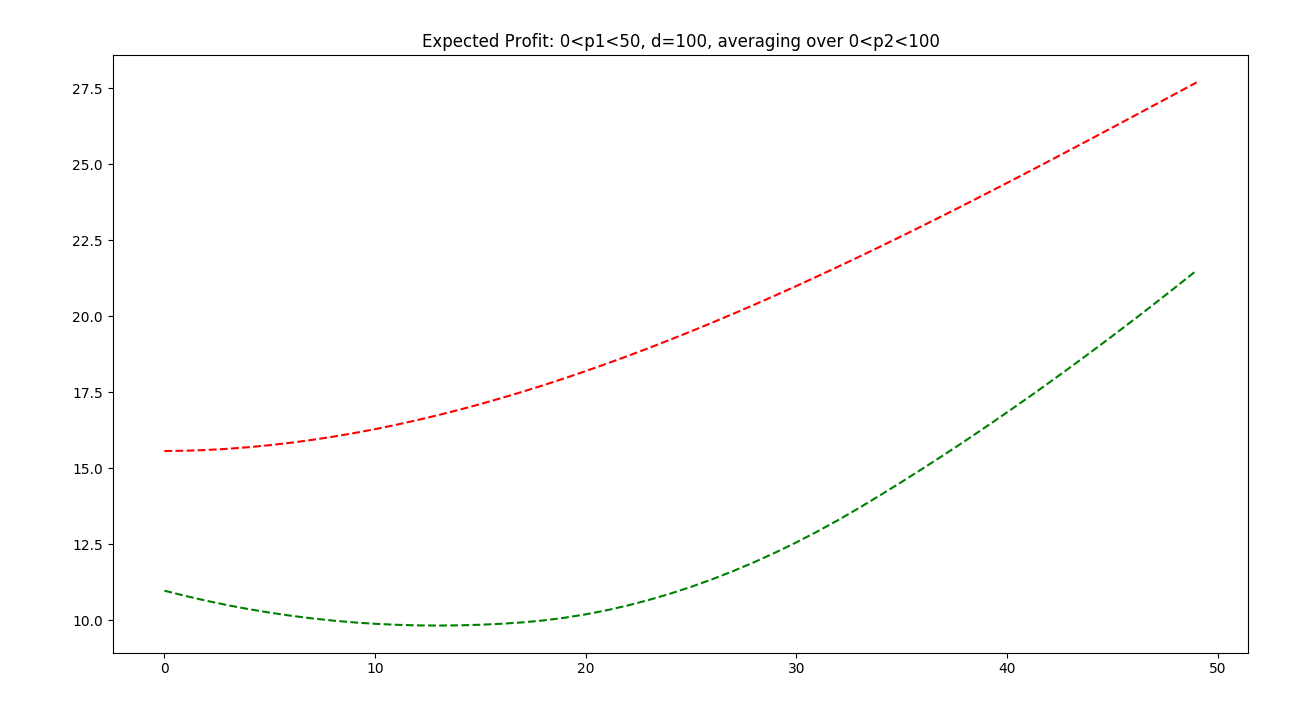
\includegraphics[width=\textwidth]{Images/E1_E2_w_wo_abs.png}
\caption{Plotting functions, \rob values vs. Expected profits, for $0<o<100$}
\label{figures: So=GF, unknown So}
\end{figure}

As we can see in Figure \ref{figures: So=GF, unknown So}, the expected profit for playing $\gf$ (red) is always greater than that of playing \gn (green)
}

\end{caseof}


\subsection{Problem 4 - Zero Information}
The last and least interesting case is the zero-information case. We would like to know what is the best $S_{\rob}$ when \rob knows nothing about \opp.
Since \rob does not now where \opp starts, it cannot play \go, and can only play \gn or \gf. Should \rob play as if no opponent exists, or should it take in consider its existence?

\begin{caseof}
  \case{Ignore \opp's existence}
  {Let \rob first assume that \opp does not exists. If that is the case, it simply wants to cover all of \w as fast as possible (with the least repetitions). In order to do so, \rob will choose $S_{\rob} = \gn$}, as it was shown to hold this condition. 
  Notice that in here, we want to minimize the amount of time it takes \rob to cover all of \w, and we do not care about \opp's existence and what it does. This may not be the best option, as we'll check later.
  
  \case{Consider \opp's existence}
  {
  Here, we do consider \opp's existence, and trying to find the profit under this assumption. The profit  depends heavily on $S_{\opp}$ and $i_{\opp}$. 
  One need to consider the two different options \gn and \gf, and then integrate over all possible options for $i_\rob$, to get the relevant expected profit \fcc.
  Let us consider what we learned in \ref{subsections: 1D, known strategy, hidden position}. There, we showed that for different strategies of \opp, it always better to play \gf. Since we showed it for both options of $S_\opp$, we use it here and say that when having zero-information regarding \opp, the best thing to do is play \gf. 
  }
\end{caseof}

Taking the above in consideration, it obvious that taking \opp's existence in consideration is better, as is shown in figures (), and therefore \rob should play \gf when having zero information regarding \opp.


\subsection{Symmetric Knowledge}
Up to this point, we considered the asymmetrical knowledge problem: we assumed different information models for \rob over \opp, but in all of them it knows of \opp's existence.
In all of these models, we assumed that \opp does not know about \rob existence (at least until meeting it). We checked different options for $S_{\opp}$, even though a rational player would just select strategy \gn (since its goal it to cover all the area, in the minimal time).

In this part, let us try and analyze the game when \opp has the same information model as \rob.
\subsubsection{Symmetrical Perfect Information}
Here, each player knows all about their opponent: both \rob and \opp knows about their opponents existence, their initial position and their strategy.
Recall that in the equivalent asymmetrical case, \rob chose playing \go, and we proved the optimality of this.

Now, assume that \opp knows \rob's strategy, and now has the opportunity to choose how to play in response: since it wants to maximize its \fcc, and it knows that when it'll meet \rob, \rob will turn and go toward the edge in its horizon, \opp will try and maximize the number of cells it cover before meeting with \opp, since from their behaviors we knows that after meeting with each other, each one will cover the cells left in its side of \w. In order to maximize this, \opp will go toward $i_{\rob}$, \rob's initial position, until meeting, then turn around and cover whats left - \go.

All we said above is regardless as to what strategy \rob is choosing, and all of it stands on the claim that regardless to $S_{\rob}$, $S_{\opp}$ will still choose as said above. The proof of correction mostly depends on what we say earlier, in the asymmetrical, full information, problem: we showed that both when $S_{\opp}=\gn$ and when $S_{\opp}=\gn$, \rob's best strategy is the same, going toward it first. Since this whole problem is symmetrical (in the sense of \rob and \opp roles, not the information symmetry we are discussing), this also applies to our case.
Therefore, there is only one case left, where the opponent goes toward us. This we explained above, and are left to formally prove it (in the same way as in \ref{subsections: full and partial information, 1D world}).


This whole logic is also valid now for \rob choice; Assume that \rob knows $S_{\opp}$: it knows that \opp will choose to  go toward $i_{\rob}$ in order to covers as much cells as it can before meeting with it. \rob has two options now: go far from \opp or go toward it: since the world from $i_{\rob}$ to the far side of \opp is 'guaranteed' to it, it prefers as much as it can from whats left, thus \rob will first go toward $i_{\opp}$ and covers as much as it can, turn around at the meeting point, and go and cover it's side of the world.

These strategies form a Nash-Equilibrium, where no player wants to change strategy given that the other player does not change it.

The profit is then very simple to compute:
Each player covers half the cells between its initial position and the opponent's initial position, then go back and covers the cells to the far side of its opponent (the distance of its initial position and the respective edge of the world \w).
Considering the setting we used above (where w.l.o.g \rob is to the  left of \opp), \rob's profit will be:\[\fcc_r=\frac{\abs*{i_{\opp} - i_{\rob}}}{2}+\abs*{i_{\rob}-0}\] and \opp's profit will be: \[\fcc_{\opp}=\frac{\abs*{i_{\opp} - i_{\rob}}}{2}+\abs*{\w - i_{\opp}}\]

Averaging over the optional initial positions $i_{\rob}$ and $i_{\opp}$ will yield:

\[E\left[\fcc_{\rob}\right]=\int_{0}^{\frac{\w}{2}}{\frac{i_{\opp} - i_{\rob}}{2}+i_{\rob}} \, di_{\rob} di_{\opp}=\frac{\w^3}{8}=\int_{0}^{\frac{\w}{2}}{\frac{i_{\opp} - i_{\rob}}{2}+\w-i_{\opp}} \, di_{\rob} di_{\opp}=E\left[\fcc_{\opp}\right]\]

The symmetry confirms the w.l.o.g. assumptions and the Nash-Equilibrium we found.

\subsubsection{Symmetrical Partial Information - Known Initial Position and Hidden Strategy}
The case here is already known from the previous one: there, we assumed different strategies for the opponent and showed that the best response was to play as explained. Since for all options that behavior was the same, we extend this result directly to here and say that in this case also, the best response for \textbf{both} players, each of them knows only their opponent's initial position but not strategy, would be to go toward it until meeting it, then turn around and go back to cover whats left.
The profit and expected profit will be the same.

\subsubsection{Symmetrical Partial Information - Hidden Initial Position and Known Strategy}

\subsubsection{Symmetrical Zero Information}
In the asymmetric-information case, in order to maximize the averaged \fcc, \rob choose $S_\rob=\gf$.
Here, in the same way as before, we would like to find a Nash-Equilibrium for the case where both players know about their opponent existence, but nothing else.
Our first and most obvious choice will be $\lbrace \gf, \gf \rbrace$, follows directly from the symmetrical case.
The proof is pretty simple: assuming that $S_\opp = \gf$, \rob does not want to switch from \gf to \gn, as known from \ref{subsections: 1D, known strategy, hidden position}. This also the case when $S_\opp=\gf$.
Since both players have symmetrical information, one can change between \rob and \opp, finishing the proof. (\todo






\newpage
\section{2D World}
Up to this point we consider \w to be the simplest: only one dimension, with nearly perfect initial information for \rob about \opp. We will now make things a bit more interesting, by considering a more realistic, 2D world.
\subsection{Complete-Information}
In this section we consider the case in which \rob has complete information on \opp's initial location and strategy, and describe an optimal strategy for \rob that first maximizes $\textnormal{\fcc}_r$, then minimizes the covering time. We show that a simple algorithm, \textbf{GIPC},  that finds first the quickest interception point with \opp's path, and then plays $S_{\opp}$, is optimal.
%We claim that the following algorithm does so: Find the closest interception point. Go there, and from there play $S_{\opp}$. Since \rob Go to Interception point, then Copy, lets call it \textbf{GIPC}. Note that \textbf{GIPC} is sane.

\begin{algorithm}
\begin{algorithmic}
	\STATE $i_p^{S_{\rob} S_{\opp}} \leftarrow $ Find Interception Point between $S_{\rob}$ and $S_{\opp}$
    \STATE GoTo $i_p^{S_{\rob} S_{\opp}}$, precede \opp by one step
    \LOOP
    	\IF {Cell $c_i$ \NOT Covered already}
        	\STATE GoTo $S_{\opp}(c_i)$
        \ENDIF
    \ENDLOOP
  
\end{algorithmic}
\caption{GIPC\label{lss}}
\end{algorithm}

\subsubsection{\textbf{GIPC} - Optimality proof}\label{subsection:GIPC, optimality proof}
We now prove that \textbf{GIPC} maximizes $\textnormal{\fcc}_{\rob}$, given full information. 
\begin{lemma}\label{lemmas:GIPC optimality lower i_t higher FCC}
Let $S_{\opp}$ be \opp's complete algorithm. Let $S_{\rob}^1,S_{\rob}^2$ be sane algorithms for \rob, with $i_t^{S_{\opp} S_{\rob}^1}$ and $i_t^{S_{\opp} S_{\rob}^2}$ interception times, respectively. Then, if $i_t^{S_{\opp} S_{\rob}^1} < i_t^{S_{\opp} S_{\rob}^2}\Rightarrow \fcc_{\rob}(S_{\rob}^1, S_{\opp}) > \fcc_{\rob}^(S_{\rob}^2, S_{\opp})$
\end{lemma}

\begin{proof}
Let us divide the number of cells \rob and \opp are covering first to \textbf{before} and \textbf{after} the interception point. Denote by $b_r^{S_{\opp} S_{\rob}^1}$ the 'before' cells, and by $a_r^{S_{\opp} S_{\rob}^1}$ the 'after' cells. In a similar way, define $b_{\opp}^{S_{\opp} S_{\rob}^1}$ and $a_{\opp}^{S_{\opp} S_{\rob}^1}$. Notice that $\fcc_{\rob}(S_{\rob}^1, S_{\opp})=b_r^{S_{\opp} S_{\rob}^1}+a_r^{S_{\opp} S_{\rob}^1}$, and the same goes for \opp. 
Since both $S_{\rob}^1$ and $S_{\rob}^2$ are sane algorithm and work against the same algorithm $S_{\opp}$, we know that $a_0^{S_{\opp} S_{\rob}^1}=a_0^{S_{\opp} S_{\rob}^2}-\textsf{\# never-covered cells from $i_p^{S_{\opp} S_{\rob}^1}$ to $i_p^{S_{\opp} S_{\rob}^2}$}$. This means that if $i_t^{S_{\opp} S_{\rob}^1}<i_t^{S_{\opp} S_{\rob}^2}\Rightarrow a_0^{S_{\opp} S_{\rob}^1}<a_0^{S_{\opp} S_{\rob}^2}$
\\In a similar way, we can see that $b_{\opp}^{S_{\opp} S_{\rob}^1}=b_{\opp}^{S_{\opp} S_{\rob}^1}-\textsf{\# never-covered cells from $i_p^{S_{\opp} S_{\rob}^1}$ to $i_p^{S_{\opp} S_{\rob}^2}$}$, and therefore if $i_t^{S_{\opp} S_{\rob}^1}<i_t^{S_{\opp} S_{\rob}^2}\Rightarrow b_{\opp}^{S_{\opp} S_{\rob}^1}<b_{\opp}^{S_{\opp} S_{\rob}^2}$.
\\From the above, we conclude and say that $i_t^{S_{\opp} S_{\rob}^1}<i_t^{S_{\opp} S_{\rob}^2}\Rightarrow \fcc_{\opp}(S_{\rob}^1, S_{\opp})<\fcc_{\opp}(S_{\rob}^2, S_{\opp})$. And, since we know that $\fcc_{\rob}(A_?, S_{\opp})=N-\fcc_{\opp}(A_?, S_{\opp})$, it obviously mean than that $i_t^{S_{\opp} S_{\rob}^1}<i_t^{S_{\opp} S_{\rob}^2}\Rightarrow \fcc_{\rob}(S_{\rob}^1, S_{\opp})>\fcc_{\rob}(S_{\rob}^2, S_{\opp})$.
\end{proof}


\begin{lemma}\label{lemmas: bound on interception time}
Suppose that \w is obstacles-free square grid of size $N\geq 16$, and both $S_{\rob}$ and $S_{\opp}$ are optimal coverage strategies, then if $S_{\rob}$ want to minimize the interception time, $i_t^{S_{\opp} S_{\rob}}$, then $i_t^{S_{\opp} S_{\rob}}\leq \frac{N}{2}$.
\end{lemma}
\begin{proof}
For a rectangular world of size $\sqrt{N} \times \sqrt{N}$, the longest path \rob can go until reaching $i_p^{S_{\opp} S_{\rob}}$ is $\sqrt[]{N}+\sqrt[]{N}$ (the length of the rectangle's diagonal). For our assumption to hold, $N$ should follow: \[2\sqrt[]{N}\leq \frac{N}{2}\Rightarrow N\geq 16 \]
%Assuming there are more than 16 cells in \w is a reasonable assumption, completing our proof.
\end{proof}

\begin{lemma} \label{lemmas: GIPC optimality prefer S with i_p}
Let $S_{\opp}$ be \opp's coverage algorithm, and let $S_{\rob}^1$ be \rob's algorithm s.t. $\nexists i_p^{S_{\opp} S_{\rob}^1}$, then if $\exists S_{\rob}^2$ s.t. $S_{\rob}^2$ is sane and $\exists i_p^{S_{\opp} S_{\rob}^2}\Rightarrow \exists S_{\rob}^{\star}$ s.t. $S_{\rob}^{\star}$ is sane and $\fcc(S_{\rob}^1, S_{\opp}) < \fcc(S_{\rob}^{\star}, S_{\opp})$.
\end{lemma}

\begin{proof}
%In order to prove the above, let us first prove the following claim: 
Following Lemma \ref{lemmas: bound on interception time}, since $i_t^{S_{\opp} S_{\rob}}$, then in worst case scenario we get $\fcc_{\opp}(S_{\rob}, S_{\opp})=
\frac{N}{2}$. However, this means that $\fcc_{\rob}(S_{\rob}, S_{\opp})=\frac{N}{2}$, and for every algorithm with interception time \textbf{lower} than $i_t^{S_{\opp} S_{\rob}}$, we get \textbf{lower} $\fcc_{\opp}$ and \textbf{higher} $\fcc_{\rob}$, thus completing the proof.
\end{proof}

\begin{theorem}\label{theorems:FullInformationStrategy}
Let $S_{\opp}$ be some complete coverage algorithm for \opp. Let $S_{\rob}$ be a sane coverage algorithm for \rob, then if $S_{\rob}$ minimizes $i_t^{S_{\opp} S_{\rob}}$ the it is optimal for \rob. i.e. $S_{\rob}$ maximizes $\fcc_{\rob}(S_{\rob}, S_{\opp})$.
\end{theorem}
\begin{proof}
This follows directly from Lemmas \ref{lemmas:GIPC optimality lower i_t higher FCC}  and \ref{lemmas: GIPC optimality prefer S with i_p}: Since \rob goes directly toward the interception point, and from there, plays $S_{\opp}$ as $S_{\rob}$(\ref{lemmas: GIPC optimality prefer S with i_p}), and then we would like to find the earliest interception point possible, since it would yield the the highest $\fcc_{\rob}(S_{\rob}^\star, S_{\opp})$ possible (\ref{lemmas:GIPC optimality lower i_t higher FCC}).
\end{proof}

\subsubsection{Best-Case and Max-Min}
In the previous subsection \ref{subsection:GIPC, optimality proof}, we considered \fcc to be our target function, and we tried to maximize it. In other information models, we'll look at $\mathbb{E}[\fcc]$ instead of only \fcc, averaging on different values, according to the relevant known information.
But there are other criteria we can take in consideration in order to assess the qualities of one strategy or another.
We now consider two new criteria: best case and max-min.
In the \textbf{best case}, \rob starts in the interception point. From there, it has no path to go before starting to intercept \opp, thus \[\max[\fcc] = m\cdot n-1\] where $m,n$ are the width and height of our world.
In the \textbf{worst case}, \rob needs to walk the max number of cells before reaching the interception point, which is the sum of the width and height of our world \w. The worst case leads to profit of: \[\min[\fcc] = m\cdot n - \sqrt{m^2 + n^2} - 1\]

We claim that GIPC maximizes both the best-case and max-min criteria. The proof for the first is trivial, and for the second is easy to show after knowing lemma \ref{lemmas:GIPC optimality lower i_t higher FCC}, and is left to the reader.


\subsubsection{Expected Profit - Exact calculation}
In \ref{subsection:GIPC, optimality proof}, we proved the optimality of GIPC. It derive directly GIPC also maximizes $\mathbb{E}[\fcc]$. Using this strategy, the profit for each game is the size of the world $N$, minus the number of steps it takes for \rob to reach the interception point $i_p$.
Since $N$ is constant, and according to the rules of expected value, the total expected \fcc is: \[\mathbb{E}\left[\fcc\right]=N-\mathbb{E}\left[i_p^t \Leftrightarrow\textnormal{steps to interception point}\right]\]

Where: \[\mathbb{E}\left[i_p^t\right]=\sum_{s}{s\cdot P\left(i_p^t=s\right)}\]
Since both \rob and \opp initial positions are uniformly distributed over the world, and have any optimal coverage algorithm, we can say that computing the expected distance to interception point is equal to computing the expected distance between two cells on the grid.

\begin{lemma}\label{lemmas:ExpectedDistanceTwoCellsRectangular}
The expected distance between two cells on a rectangular grid of size $m\times n$ is \[\frac{\left(m+1\right)\left(m-1\right)}{3m}-\frac{\left(n+1\right)\left(n-1\right)}{3n}\] 
\end{lemma}
\begin{proof}
Consider $X_1,Y_1,X_2,Y_2$ to be random variables, indicating the coordinates for cell $C_1=\lbrace X_1, Y_1 \rbrace$ and  cell $C_2=\lbrace X_2, Y_2 \rbrace$. Each coordinate, can fall anywhere in the range $\left[1\ldots m\right]$.
The expected distance between two cell is:
\[\mathbb{E}\left[\abs*{C_2-C_1}\right]=\mathbb{E}\left[\abs*{X_2-X_1} + \abs*{Y_2-Y_1}\right]=\mathbb{E}\left[\abs*{X_2-X_1}\right]+\mathbb{E}\left[\abs*{Y_2-Y_1}\right]\]

Let us compute the first part first:

% The calculation o $\mathbb{E}\left[\abs*{X_2-X_1}\right]$ is equal to the calculation of $ \mathbb{E}\left[\abs*{Y_2-Y_1}\right]$, except for the range on which the variables are distributed over, let us compute just the first one, and deduce the second right after:
\begin{multline*}
\mathbb{E}\left[\abs*{X-Y}\right] = \\
\sum_{x=1}^{m}\sum_{y=1}^{m}{\frac{\abs*{x-y}}{m^2}} = \sum_{x=1}^{m}\sum_{y=1}^{x}{\frac{x-y}{m^2}}+\sum_{x=1}^{m}\sum_{y=x+1}^{m}{\frac{y-x}{m^2}}=\\
\frac{1}{m^2}\left(\sum_{x=1}^{m}\sum_{y=1}^{x}{x-y}+\sum_{x=1}^{m}\sum_{y=x+1}^{m}{y-x}\right)=\\
\frac{1}{m^2}\left(\sum_{x=1}^{m}{\left(x^2-\sum_{y=1}^{m}{y}\right)}\right)+
\frac{1}{m^2}\left(\sum_{x=1}^{m}\left(\sum_{y=x+1}^{m}{y}-\left(m-x\right)\cdot x\right)\right)=\\
\frac{1}{m^2}\left(\sum_{x=1}^{m}{\left(x^2-\frac{1}{2}\cdot x\left(x+1\right)\right)}\right)+
\frac{1}{m^2}\sum_{x=1}^{m}\left(\frac{1}{2}\cdot \left(m-x\right)\left(m+x+1)-\left(m-x\right)\cdot x\right)\right)=\\
\frac{1}{m^2}\sum_{x=1}^{m}{\left(x^2-\left(1+m\right)x+\left(\frac{1}{2}m^2+\frac{1}{2}m\right)\right)}=\\
\frac{m\left(\frac{1}{2}m^2+\frac{1}{2}m\right)}{m^2}+\frac{1}{m^2}\sum_{x=1}^{m}{\left(x^2-\left(1+m\right)x\right)}=\\
\frac{m+1}{2}+\frac{1}{m^2}\sum_{x=1}^{m}{x^2}-\frac{1}{m^2}\left(1+m\right)\left(\frac{1}{2}m\left(m+1\right)\right)=\\
\frac{m+1}{2}=\frac{1}{m^2}\left(\frac{1}{6}\cdot m\left(m+1\right)\left(2m+1\right)\right)-
\frac{1}{m^2}\left(1+m\right)\left(\frac{1}{2}m\left(m+1\right)\right)=\\
\frac{1}{6m}\left(3m^2+3m+2m^2+3m+1-3m^2-6m-3\right)=\\
=\frac{\left(m+1\right)\left(m-1\right)}{3m}
\end{multline*}

The second part is identical to the first, except for the range the cells are distributed over ($n$ instead of $m$). Therefore:
\[\mathbb{E}\left[\abs*{C_2-C_1}\right]=\frac{\left(m+1\right)\left(m-1\right)}{3m}+\frac{\left(n+1\right)\left(n-1\right)}{3n}\]

\end{proof}

According to \ref{lemmas:ExpectedDistanceTwoCellsRectangular}, we can finally compute the exact $\mathbb{E}[\fcc]$ over world of size $m\times n$, using GIPC as $S_{\rob}$, to be: \[\mathbb{E}\left[\fcc\right]=m\cdot n-\frac{\left(m+1\right)\left(m-1\right)}{3m}-\frac{\left(n+1\right)\left(n-1\right)}{3n}\]

\subsubsection{Experiments}
First, we tested lemma \ref{lemmas:ExpectedDistanceTwoCellsRectangular}. Using simple python code, we checked the distance between points in different world sizes. Considering a world of size $1000 \times 2000$, we expected the average distance between points to be $999.9995$. After running for 10,000,000 iterations, we got $1000.0604394$.
Doing the same check, over world of size $500\times 3000$, expecting to get $1166.66588889$, we got $1166.8190994$. Again, a considerably correct result.

Next, we wanted to test the expected profit, when $S_{\rob} = GIPC$. For that, we ran simulations (with agents and behaviors), over world of size $100 \times 100$, expecting the results to be $9933.34$.
The average gain we got is $9933.613$.

The simulation process is described in algorithm \ref{algorithms:GIPC simulations}
\begin{algorithm}
\begin{algorithmic}
    \FOR {x=100000 iterations}
    	\STATE Choose $i_{\opp}\in \left[0,99\right]$ in random
        \STATE Choose $i_{\rob}\in \left[0,99\right]$ in random
        \STATE Choose $S_{\opp}\in \mathcal{S}$ in random
        \STATE $S_{\rob} \leftarrow GIPC\left(S_{\opp}, i_{\opp}\right)$
    	\STATE sum $\leftarrow $ sum$+ {\fcc}_{\rob}(S_{\rob},S_{\opp}, i_{\rob}, i_{\opp})$
    \ENDFOR
    \RETURN sum$/x$
  
\end{algorithmic}
\caption{Simulation, Full Knowledge, using GIPC\label{algorithms:GIPC simulations}}
\end{algorithm}


\subsection{Zero-Knowledge Case}\label{subsubsections:ZeroKnowledge}
In this part we try to investigate the case where \rob has zero knowledge regarding \opp (except for the fact that it exists). We would like to know what is the best strategy to do, considering the different measurement methods.

\begin{definition}[\textbf{CROS}]
Let \textbf{\cros} (Choose Random Optimal Strategy) be a strategy where one select some random optimal covering algorithm, and plays it from the start. 
\end{definition}

\subsubsection{Best Case and Min-Max}
Let us first analyze \cros in terms of best-case and min-max:
The best case one can achieve by playing \cros is $N-1$ - happens when $S_{\rob} = S_{\opp}$, and \rob and \opp start right next to each other; That is, \rob precede \opp by exactly one cell, and have the same strategy.
The worst case leads to profit of $1$, and happens when \opp precedes \rob by exactly one cell.

\textcolor{blue}{Is that of any interest to us?}

\subsubsection{Expected Profit}
We assume, and will show next, that when having zero knowledge regarding \opp, if \rob is playing \cros its maximizes $\mathbb{E}[\fcc]$

\begin{lemma}\label{lem:NoInformationEFCC}
When having zero-information regarding \opp, by playing \textbf{\cros} \rob maximizes the $\mathbb{E}\left[\fcc\right]$ and minimizes the covering time.
\end{lemma}

To prove that, let us first investigate the probability for loss and gain by \rob over some cell $c_i$ at some time $T$.
The probability $P\left(\textnormal{$c_i$ is covered by this step $T$}\right)$ consists of the probability that \opp is covered after exactly $T$ steps (i.e. it covered at this step), or the probability it was covered the step before (i.e. after $T-1$), and so on, up to $t=1$, which is the probability that \opp started at $c_i$, and therefore covered it.
We therefore denote the probability for this by:
\[P\left(\textnormal{$c_i$ is covered by step $T$}\right)=\sum_{t=1}^{T}{P\left(\textnormal{$c_i$ was covered after exactly $t$ steps}\right)}\]


The reader can easily see the correctness of the next lemma:
\begin{lemma}\label{lemmas:ProbThroughTime}
$P\left(\textnormal{$c_i$ is covered by step $t_1$}\right)>P\left(\textnormal{$c_i$ is covered by step $t_2$}\right)$ iff $t_1>t_2$.
\end{lemma}

We can use this definition, and now prove lemma \ref{lem:NoInformationEFCC}, the no information case:

\begin{proof}
First, since \rob is playing an optimal-coverage algorithm, it's by definition minimizes the covering time.
Second, let us prove that playing an optimal-coverage from the beginning, maximizes the $\mathbb{E}[\fcc]$ target function. We will prove that by showing that at any step, taking an already covered cell hamper the total expected gain of the coverage path.
Consider some time $t=k$, where \rob has 4 options where to go to (recall that we are assuming Von Neumann neighborhood), and assume that at least one of these neighbors are already covered cell.
Now, let us look at the $\mathbb{E}[\fcc]$ function: if \rob is taking an unvisited cell, its $\mathbb{E}[\fcc]$ is:
\[\mathbb{E}[\fcc]_{unvisited}=\frac{1}{N}\cdot \sum_{t=1}^{N}\left(1-P\left(\textnormal{$c_i$ is covered by step $t$}\right)\right)\]

where if it takes the already visited cell its $\mathbb{E}[\fcc]$ is: 
\begin{multline*}
\mathbb{E}[\fcc]_{visited}=\frac{1}{N}\cdot \sum_{t=1}^{k-1}\left(1-P\left(\textnormal{$c_i$ is covered by step $t$}\right)\right) + \frac{1}{N}\cdot \sum_{t=k+1}^{N+1}\left(1-P\left(\textnormal{$c_i$ is covered by step $t$}\right)\right)
\end{multline*}
Notice that if \rob takes the already covered cell, since it covers all the cells in the world (the algorithm is defined as complete one), it must go through $N-k$ more cells, but it does so in a 'phase' of $1$ in time: that is, the $k$'th cell is covered in time $k+1$ and so on.
Now, according to lemma \ref{lemmas:ProbThroughTime}, it goes that $\sum_{t=k+1}^{N+1}\left(1-P\left(\textnormal{$c_i$ is covered by step $t$}\right)\right) < \sum_{t=k}^{N}\left(1-P\left(\textnormal{$c_i$ is covered by step $t$}\right)\right)$, and therefore the expected \fcc that \rob gains by visiting an unvisited cell is higher than by that it gains by visiting an already-visited cell.
It therefore true that any algorithm which wants to maximizes the $\mathbb{E}[\fcc]$ must not visit the same cell twice. Since this refers exactly to any optimal-coverage algorithm, we finished proving that playing an optimal-complete-coverage algorithm from the start does minimizes the $\mathbb{E}[\fcc]$, and therefore optimal.
\end{proof}


Next, we'll show that this strategy yields us $\mathbb{E}[\fcc]=\frac{N}{2}$. The next lemma has been shown to be true by experiments (the algorithm will be explained in the experiments subsection \ref{subsubsections:ZeroKnowledgeExpreiments})

\begin{lemma}\label{lemmas:ZeroKnowledgeEFCC}
When having zero-information, $S_{\rob}=\textbf{\cros}$ yields $\mathbb{E}[\fcc_{\rob}]=\frac{N+1}{2}$.
\end{lemma}

\begin{proof}
To prove, first notice the following: for cell $c_i$ at time $i$, we say that $c_i$ is 'gained' by player \rob \textbf{iff} its covering-time (by $S_o$) value (the time it was first covered by robot \opp) - ${CT}_{\opp}(c_i)$ - is higher than the time it was covered by robot $\rob$ - ${CT}_{\rob}(c_i)$.
Now, we can re-write the expression for \rob's gain to use property of covering time: \[\mathbb{E}[\fcc]=\mathbb{E}\left[\sum_{i=1}^{N}{\mathds{1}\left[CT\left(c_i\right)\geq {CT}_{\rob}(c_i)\right]}\right]\]
Using the expectation rules, we can insert the expectation sign inside the summation: \[\mathbb{E}[\fcc]=\sum_{i=1}^{N}{\mathbb{E}\left[\mathds{1}\left[{CT}_{\opp}(c_i)\geq {CT}_{\rob}(c_i)\right]\right]}\]

So now, let us prove that $\mathbb{E}\left[\mathds{1}\left[{CT}_{\opp}(c_i)\geq {CT}_{\rob}(c_i)\right]\right]=\frac{1}{2}$. 
Using Markov's inequality, we know that: \[\mathbb{E}\left[\mathds{1}\left[{CT}_{\opp}(c_i)\geq {CT}_{\rob}(c_i)\right]\right]=P\left({CT}_{\opp}(c_i)\geq {CT}_{\rob}(c_i)\right)\]
So we need to prove that the probability for the covering-time of some cell $c_i$ by $S_{\opp}$ to be greater than some constant value ${CT}_{\rob}(c_i)$, where ${CT}_{\rob}(c_i)$ is uniform in range $[0,1]$, is equal to $\frac{1}{2}$.
Indeed, this is true, and here is why: both ${CT}_{\opp}(c_i)$ and ${CT}_{\rob}(c_i)$ are considered as i.i.d variables, each one of them is uniformly distributed between $0$ and $N$. Then, the probability that one is greater than the other is $\frac{1}{2}$, as can be deduced from the following graph, indicating all the cases where ${CT}_{\opp}(c_i) > {CT}_{\rob}(c_i)$:

  
     \begin{figure}[thpb]
      \centering
      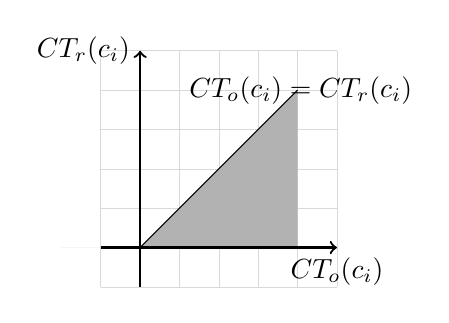
\begin{tikzpicture}
    \draw[very thin, gray!30, step=0.5 cm](-0.5,-0.5) grid (2.5,2.5);

    \fill [gray!60, domain=0:2, variable=\x]
      (-1, 0)
      -- plot ({\x}, {\x})
      -- (2, 0)
      -- cycle;

    \draw [thick] [->] (-0.5,0)--(2.5,0) node[right, below] {$CT_{\opp}(c_i)$};
%      \foreach \x in {-0.5,...,1}
%        \draw[xshift=\x cm, thick] (0pt,-1pt)--(0pt,1pt) node[below] {$\x$};

    \draw [thick] [->] (0,-0.5)--(0,2.5) node[above, left] {$CT_{\rob}(c_i)$};
%      \foreach \y in {-0.5,...,2}
%        \draw[yshift=\y cm, thick] (-1pt,0pt)--(1pt,0pt) node[left] {$\y$};

    \draw [domain=0:2, variable=\x]
      plot ({\x}, {\x}) node[right] at (0.5,2) {$CT_{\opp}(c_i)=CT_{\rob}(c_i)$};

  \end{tikzpicture}
      \caption{Inductance of oscillation winding on amorphous
       magnetic core versus DC bias magnetic field}
      \label{figurelabel}
   \end{figure}
  
Using the above, we get that:
\[\mathbb{E}[\fcc]=\sum_{i=1}^{N}{\mathbb{E}\left[\mathds{1}\left[CT\left(c_i\right)\geq i\right]\right]}=\sum_{i=1}^{N}{\frac{1}{2}}=\frac{N+1}{2}\]
\end{proof}

\subsubsection{Experiments}\label{subsubsections:ZeroKnowledgeExpreiments}
Using simulations, we found that our expectations were true, and indeed the iterations we ran, the closer the expected gain was to $\frac{N+1}{2}$.

The Algorithm we used is as follows:

\begin{algorithm}
\begin{algorithmic}
    \FOR {x=100000 iterations}
    	\STATE Choose $i_{\opp} \in \left[0,99\right]$ in random
        \STATE Choose $i_{\rob} \in \left[0,99\right]$ in random
        \STATE Choose $S_{\opp} \in \mathcal{S}$ in random
        \STATE $S_{\rob} \leftarrow \cros\left(\right)$
    	\STATE sum $\leftarrow $ sum$+ {\fcc}_{\rob}(S_{\rob},S_{\opp}, i_{\rob}, i_{\opp})$
    \ENDFOR
    \RETURN sum$/x$
  
\end{algorithmic}
\caption{Simulation, Zero Knowledge\label{algorithms:zero knowledge, simulations}}
\end{algorithm}


\subsection{Known Strategy, Hidden Initial Position}
\subsubsection{our Chosen algorithm, and optimality proof (need refining!)}
As our problem progress, we have many strategies, each has an advantage when considering different measurement methods. 
Beside \textbf{\cros}, let us define the main strategy that will be investigated in this part:
\begin{definition}[\textbf{\coos}]
Let \textbf{\coos} (Choose Opponent's Strategy) be strategy where \rob selects the opponents strategy $S_{\opp}$, and plays it from the beginning.
\end{definition}

\subsubsection{Max-Min}
For both \textbf{CRS} and \textbf{COS}, it holds that: \[\max\mathbb{E}[\fcc]=m\cdot n-1, \min\mathbb{E}[\fcc]=1\]

\subsubsection{Expected Profit}

\paragraph*{\cros}

From simulations, we know that playing \cros yields expected profit of $\frac{m\cdot n+1}{2}$. We claim and prove that when considering the expected profit while averaging the initial position of \opp, the above is true for any two optimal strategies.
\begin{theorem}\label{theorems:expected FCC, only So known}
Let $S_{\opp}$, $i_{\opp}$ denote the coverage strategy and initial position of \opp, respectively. In a similar way, denote $S_{\rob}$ and $i_r$. \rob is given only $S_{\opp}$. Then, it holds that $\mathbb{E}\left[\fcc\left(S_{\rob}, i_r, S_{\opp}, i_{\opp}\right) \mid S_{\rob}, i_r, S_{\opp}\right]=\frac{m\cdot n+1}{2}$. That is, averaging over $i_{\opp}$ yields expected \fcc of $\frac{m\cdot n+1}{2}$.
\end{theorem}
\begin{proof}
First of all, let us define covering time: 
\begin{definition}[\textbf{Covering-Time}]
the Covering-Time of cell $c_i$ by \rob, using the coverage strategy $S_{\rob}$ is the time \rob first visits $c_i$, according to $S_{\rob}$. This value is denoted by ${CT}_{S_{\rob}}(c_i)$.
\end{definition}
Now, since $S_{\rob}$ and $S_{\opp}$ are optimal-cyclic-coverage strategies, which means they start and stop at the same position, visiting each cell exactly once (since we assume a rectangular world with no obstacles, such a path exists). We can say that each strategy create a 'chain' from all the cells in the world $c_0,...,c_{N-1}$. In this chain, the relative place a cell $c_i$ appears in is its ${CT}_{S_{\rob}}(c_i)$ (We are talking about \rob,  from now on, but all of this is the same for \opp). Here is an illustration of our covering-chains:
\begin{figure}
\centering
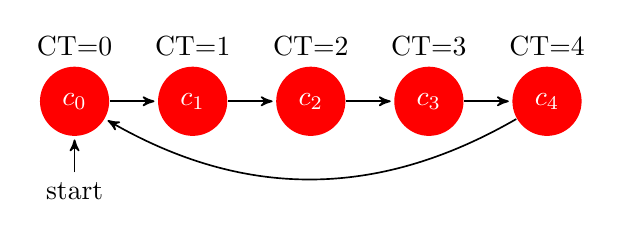
\begin{tikzpicture}[->,>=stealth',shorten >=1pt,auto,node distance=1.5cm,
                    semithick]
  \tikzstyle{every state}=[fill=red,draw=none,text=white]

  \node[initial below,state, label={CT=0}] (A)              {$c_0$};
  \node[state, label={CT=1}]         (B) [right of=A] {$c_1$};
  \node[state, label={CT=2}]         (C) [right of=B] {$c_2$};
  \node[state, label={CT=3}]         (D) [right of=C] {$c_3$};
  \node[state, label={CT=4}]         (E) [right of=D] {$c_4$};

  \path (A) edge              node {} (B)
        (B) edge              node {} (C)
        (C) edge              node {} (D)
        (D) edge              node {} (E)
        (E) edge [bend left] node {} (A);
\end{tikzpicture}

\caption{An example for a covering chain, where coverage path starts at $c_0$}
\end{figure}


Now, understand this: each starting position $i_r$ determines the covering time of all the cells $c_0,...,c_{N-1}$; Since we assumed the strategy is known before hand, then, for \opp,  the covering time is set after $i_{\opp}$ is known, and changing it changes for all the cells their covering time. Here is an illustration:

\begin{figure}
\centering
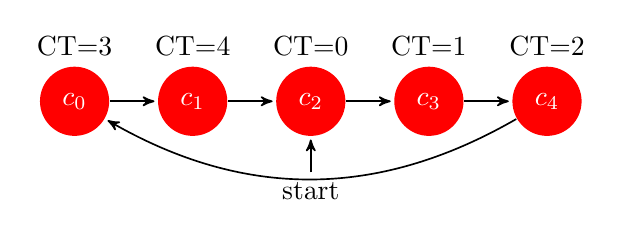
\begin{tikzpicture}[->,>=stealth',shorten >=1pt,auto,node distance=1.5cm,
                    semithick]
  \tikzstyle{every state}=[fill=red,draw=none,text=white]

  \node[state, label={CT=3}] (A)              {$c_0$};
  \node[state, label={CT=4}]         (B) [right of=A] {$c_1$};
  \node[initial below,state, label={CT=0}]         (C) [right of=B] {$c_2$};
  \node[state, label={CT=1}]         (D) [right of=C] {$c_3$};
  \node[state, label={CT=2}]         (E) [right of=D] {$c_4$};

  \path (A) edge              node {} (B)
        (B) edge              node {} (C)
        (C) edge              node {} (D)
        (D) edge              node {} (E)
        (E) edge [bend left] node {} (A);
\end{tikzpicture}

\caption{An example for a covering chain, where coverage path starts at $c_2$.}
\end{figure}
As can be seen in the examples above, changing $i_{\opp}$ directly changes the Covering-Time values of all vertices accordingly.
As the reader can see, since $S_{\opp}$ is set, then for any $c_i$ we'll get $CT_{S_{\opp}}(c_i)=0$ if $i_{\opp}=c_i$, and $CT_{S_{\opp}}(c_i)=N-1$ if $i_0=c_{N-1}$. More generally: if $i_{\opp}=c_j$ where $j$ ranges from $0$ to $N-1$, then $CT_{S_{\opp}}(c_i)=\abs{i-j}\in [0,N-1]$.

We now move to the next part: converting the way we look on \fcc. As seen before, one can write the \fcc of a fixed problem (with all its variables known) as $\fcc(W,S_{\rob},S_{\opp},i_r,i_{\opp})=\# \lbrace CT_{S_{\rob}}(c_i) \le CT_{S_{\opp}}(c_i)\rbrace \textsl{ where } c_i\in W$.
If before we wanted to find the expected \fcc expression: 
\[\mathbb{E}\left[\fcc\left( S_{\rob}, i_r, S_{\opp}, i_{\opp}\right) \mid S_{\rob}, i_r, S_{\opp}\right]=
\frac{1}{N}\sum_{i_{\opp}\in W}{\fcc\left(W,S_{\rob},i_r,S_{\opp},i_{\opp}\right)}\]
We now consider the following expression instead:
\[\mathbb{E}\left[\fcc\left( S_{\rob}, i_r, S_{\opp}, i_{\opp}\right) \mid  S_{\rob}, i_r, S_{\opp}\right]=
\frac{1}{N}\sum_{i_{\opp}\in W}{\sum_{c_i\in W}{\mathds{1}\left[CT_{S_{\rob},i_r}(c_i) \le CT_{S_{\opp},i_{\opp}}(c_i)\right]}}\]

If we change the order of summation, we can use what we know about ranging over the initial position and get:
\begin{multline*}
\mathbb{E}\left[\fcc\left(W, S_{\rob}, i_r, S_{\opp}, i_{\opp}\right) \mid W, S_{\rob}, i_r, S_{\opp}\right]=\\
\frac{1}{N}\sum_{i_{\opp}\in W}{\sum_{c_i\in W}{\mathds{1}\left[CT_{S_{\rob},i_r}(c_i) \le CT_{S_{\opp},i_{\opp}}(c_i)\right]}}= \\
\frac{1}{N}\sum_{c_i\in W}{\sum_{i_{\opp}\in W}{\mathds{1}\left[CT_{S_{\rob},i_r}(c_i) \le CT_{S_{\opp},i_{\opp}}(c_i)\right]}}=\\
\frac{1}{N}\sum_{c_i\in W}{\# \lbrace CT_{S_{\rob},i_r}(c_i) \le CT_{S_{\opp},i_{\opp}}(c_i)\rbrace}=\\
\frac{1}{N}\sum_{c_i\in W}{N-CT_{S_{\rob},i_r}(c_i)}=\\
\frac{1}{N}(1+2+\ldots+N)=\frac{N+1}{2}
\end{multline*}
Where the before-last equation comes from what we said we before: the number of times that $CT_{S_{\opp},i_{\opp}}(c_i)$ is greater or equal to $CT_{S_{\rob},i_r}(c_i)$ (can be considered as some constant $C$), when ranging over all cells as $i_{\opp}$, ranges itself from $N$ (if $i_{\opp}$ is exactly one cell after $c_i$) to $1$ (if $i_{\opp}$ is exactly one cell before $c_i$).


\end{proof}
As theorem \ref{theorems:expected FCC, only So known} clearly indicates, it works for any two optimal strategies. Thus, we conclude and say that the optimal solution in this knowledge is case is as good as the worst solution, since when averaging over $i_{\opp}$, we get expected \fcc of $\frac{N+1}{2}$.

\paragraph*{COS}

\begin{lemma}\label{theorems: only So is known, COS, EFCC}
Consider the case where \rob knows only \opp's strategy, but not its position. Then, playing \textbf{COS} yields $\mathbb{E}\left[\fcc\right]=\frac{N+1}{2}$.
\end{lemma}

Lemma \ref{theorems: only So is known, COS, EFCC} is a specific case of CRS (where we proved this to all strategies), but the proof (even though is redundant now) is very simple and intuitive.

\begin{proof}
Denote the coverage path \opp is doing by $C=\lbrace(c_0=i_{\opp}),c_1,...,c_{N-1}\rbrace$. $i_{\rob}$ is some unknown cell, let's say $i_{\rob}=c_k \in A$. Since $S_{\rob}=S_{\opp}$, then \rob visits first all the cells from its initial position $i_r=a_k$ to $i_{\opp}=c_0$ (not included). That is, it covers the cells $c_k,c_{k+1},\ldots,c_{N-1}$.
Since $i_{\rob}$ is uniformly distributed over \w, computing the expected profit is quite simple:

\begin{multline*}
\mathbb{E}\left[\fcc\right]=\\
\sum_{c_k\in\lbrace c_0,...,c_{N-1}\rbrace}\fcc\left(i_{\rob},C\right)\cdot P\left(i_{\rob}=c_k\right)=\\
\sum_{c_k\in\lbrace c_0,...,c_{N-1}\rbrace}\fcc\left(i_{\rob},C\right)\cdot \frac{1}{N}=\\
\sum_{c_k\in\lbrace c_0,...,c_{N-1}\rbrace}\abs*{c_{N-1}-c_k+1}\cdot \frac{1}{N}=\\
\frac{1}{N}\cdot \sum_{i=1}^{N}{i}=\frac{N+1}{2}
\end{multline*}

\end{proof}

\subsubsection{Experiments}
As before, we wanted to prove our claims in this section, using simulations of \rob and \opp behaviors.
As in this section, \rob knows $i_{\opp}$ but not $S_{\opp}$, we averaged over different options for $S_{\opp}$. The simulations method we used is shown below(\ref{algorithms:only Io known, simulations}). First, we wanted to prove our claim, that when playing random strategy, \rob do gain averaged \fcc of $\frac{N+1}{2}$. 
\begin{algorithm}
\begin{algorithmic}
	\STATE Choose $i_{\opp} \in \left[0,99\right]$ in random
    \STATE Choose $i_{\rob} \in \left[0,99\right]$ in random
    \STATE Choose $S_{\rob} \in \mathcal{S}$ in random
    
    \FOR {x=100000 iterations}
        \STATE Choose $S_{\opp} \in \mathcal{S}$ in random
    	\STATE sum $\leftarrow $ sum$+ {\fcc}_{\rob}(S_{\rob},S_{\opp}, i_{\rob}, i_{\opp})$
    \ENDFOR
    \RETURN sum$/x$
  
\end{algorithmic}
\caption{Simulation, Known $i_{\opp}$, Hidden $S_{\opp}$\label{algorithms:only Io known, simulations}}
\end{algorithm}

After that, we wanted to show that nothing better can be achieved. For this, we repeated the process above, but for different $S_{\rob}$, and saw that each one yielded expected \fcc of $\frac{N+1}{2}$. The process is explained in \ref{algorithms:only Io known, different Sr simulations}.
\begin{algorithm}
\begin{algorithmic}
	\FOR {$S_{\rob} \in \mathcal{S}$}
    	\STATE Choose $i_{\opp} \in \left[0,99\right]$ in random
          \STATE Choose $i_{\rob} \in \left[0,99\right]$ in random
      \FOR {x=100000 iterations}
          \STATE Choose $S_{\opp} \in \mathcal{S}$ in random
          \STATE sum $\leftarrow $ sum$+ {\fcc}_{\rob}(S_{\rob},S_{\opp}, i_{\rob}, i_{\opp})$
      \ENDFOR
    \RETURN sum$/x$
    \ENDFOR
    
  
\end{algorithmic}
\caption{Simulation, Known $i_{\opp}$, Hidden $S_{\opp}$, Different $S_r$\label{algorithms:only Io known, different Sr simulations}}
\end{algorithm}

Lastly, we checked that indeed, nothing is gained from using the opponent's strategy (in the simple way of playing it directly, at least). For this we simply used \ref{algorithms:only Io known, simulations}, and replaced choosing $S_{\rob}$ by random, by setting it to be $S_{\opp}$. Again, as we expected, the results where conclusive enough, and showed results of $\frac{N+1}{2}$.


\subsection{Known Initial Position, Hidden Strategy}
About this model of information, we have not a lot to say. From experiments, we know that by fixing $i_{\opp}$, and using different $S_{\opp}$, there are some strategies that are better than others, as can be shown in \textbf{figure 1 - add it!}, but we didn't find any important character of a covering-strategy that correlates with a path being good or not. We checked distance between initial positions, number of 'turns' per path, intersection with a \opp heat-map and more... but none of show direct correlation to a strategy's quality (in terms of \fcc)

\subsection{Temporary Conclusions}
This subsection will contain our conclusions, regarding this part of the research: what were the assumptions we made, what we found and what not, and what are we going to discuss next.
\section{CONCLUSIONS}

A conclusion section is not required. Although a conclusion may review the main points of the paper, do not replicate the abstract as the conclusion. A conclusion might elaborate on the importance of the work or suggest applications and extensions. 



\bibliographystyle{abbrv}
\bibliography{refs}

\end{document}











